\documentclass[
  11pt,
  a4paper,
  % titlepage,
]{article}

\title{Artificial Intelligence and Machine Learning}
\author{Martin de Spirlet}
\date{}

% Set document geometry
\usepackage[
  a4paper,
  margin = 1in,
  % showframe,
]{geometry} % Flexible and complete interface to document dimensions

% Set default font family to default sans-serif font
\renewcommand{\familydefault}{\sfdefault}

\usepackage{amsmath} % AMS mathematical facilities for LaTeX
\usepackage{amssymb} % TeX fonts from the American Mathematical Society
\usepackage{booktabs} % Publication quality tables in LaTeX
\usepackage{caption} % Customising captions in floating environments
\usepackage[inline,shortlabels]{enumitem} % Control layout of itemize enumerate description
\usepackage{graphicx} % Enhanced support for graphics
\usepackage[skip=\glueexpr\baselineskip\relax]{parskip} % Layout with zero \parindent non-zero \parskip
\usepackage[onehalfspacing]{setspace} % Set space between lines % setspace must be loaded before hyperref
\usepackage{titlesec} % Select alternative section titles
\usepackage{xcolor} % Driver-independent color extensions for LaTeX and pdfLaTeX

\PassOptionsToPackage{hyphens}{url}\usepackage{hyperref} % Extensive support for hypertext in LaTeX % hyperref loaded by pdfx

% Set list parameters (using enumitem package)
\setlist{nosep}

% Set section break command (using package titlesec)
\newcommand{\sectionbreak}{\clearpage}

% Define command for typesetting a mathematical function
\newcommand{\function}[3][]{\mathrm{#2}#1\!\left( #3 \right)}

% Increase penalty for widows and orphans (maximum 10000)
\widowpenalty = 10000
\clubpenalty = 10000

\begin{document}

\pagenumbering{gobble}

\maketitle

\vspace*{\fill}

\begin{table}[htp]
  \centering
  \begin{tabular}{rrl}
    \toprule
    Week & Unit & Title \\
    \midrule
     1 &  1 & Supervised Learning \\
       &  2 & Regression \\ [1ex]
     2 &  3 & Logistic Regression (Classification) \\
       &  4 & Neural Networks, Hyperparameters and Metrics \\ [1ex]
     3 &  5 & Na\"{i}ve Bayes \\ [1ex]
     4 &  6 & Decision Trees \\
       &  7 & \( k \)-Nearest Neighbours \\ [1ex]
     5 &  8 & Uninformed Search \\
       &  9 & Informed (Heuristic) Search \\ [1ex]
     7 & 10 & Optimisation \\ [1ex]
     8 & 11 & Evolutionary Algorithms \\ [1ex]
     9 & 12 & Reinforcement Learning \\ [1ex]
    10 & 13 & Clustering Algorithms \\
    \bottomrule
  \end{tabular}
\end{table}

\vspace*{\fill}
\addvspace{1in}

\clearpage

\pagenumbering{arabic}

\section{Supervised Learning}
\subsection{Machine Learning}

The focus of \emph{machine~learning} is the study and development of computational models capable of improving their performance with experience and acquiring knowledge by themselves.
Learning algorithms can be classified into three broad groups.
\begin{description}
  \item[Unsupervised] learning algorithms, such as the \( k \)-means algorithm, classify input data based on certain inherent properties of that data.
  \item[Supervised] learning algorithms, such as regression, logistic regression and neural networks, learn trends from annotated data in order to make predictions about previously unseen data.
  \item[Reinforced] learning algorithms learn how to achieve specific tasks in predefined environments based on rewards.
\end{description}

\subsection{Terminology and Notation}

\subsubsection{Independent and Dependent Variables}

\emph{Independent variables} take on different values based on the environment.
\emph{Dependent variables} take on values based on other variables (usually independent variables).
Dependent variables \emph{depend} on independent variables.

Dependent variables can take on continuous or discrete values.
The prediction of continuous values is known as \emph{regression}.
The prediction of discrete values or \emph{classes} is known as \emph{classification}.

For both regression and classification, a supervised learning model consists of
\begin{itemize}
  \item a hypothesis function,
  \item a cost function, and
  \item a weight update function that uses the partial differential of the cost function.
\end{itemize}

\subsubsection{Training and Test Data}

The \emph{training data} used in supervised learning are \emph{annotated} with the values of the dependent variable \( y \) for each vector \( \boldsymbol{X} \) of independent variables.
Each training datum \( i \) is of the form \( \left( \boldsymbol{X}^{(i)}, y^{(i)} \right) \).
Thus, the training data may be represented in the form
\begin{equation*}
  \left( \boldsymbol{X}^{(1)}, y^{(1)} \right), \left( \boldsymbol{X}^{(2)}, y^{(2)} \right), \ldots, \left( \boldsymbol{X}^{(N)}, y^{(N)} \right)
\end{equation*}
For each of the \( N \) training inputs \( \boldsymbol{X}^{(i)} \), the corresponding output is \( y^{(i)} \).

The \emph{test data} is an independent set of annotated data on which the trained model is tested.
While it shares the characteristics of the training data, it contains different elements.

\subsubsection{Hypothesis Function}

The \emph{hypothesis function} \( \function[_{\boldsymbol{w}}]{h}{\boldsymbol{X}} \) predicts the output \( y \) that corresponds to the input \( \boldsymbol{X} \)\@.
For regression, the general form of the hypothesis function is
\begin{equation*}
  \function[_{\boldsymbol{w}}]{h}{\boldsymbol{X}} = w_0 + w_1 x_1 + w_2 x_2 + \ldots +  w_k x_k
\end{equation*}
where \( k \) is an arbitrary number of terms (not necessarily the number of elements in \( \boldsymbol{X} \)), and each term \( x \) may be the product of any combination of elements in \( \boldsymbol{X} \)\@.

The hypothesis function is parametrised by a vector of \emph{weights} \( \boldsymbol{w} \).
The purpose of a supervised learning algorithm is to find the values of these weights for which the hypothesis function best fits the training data.

\subsubsection{Cost Function}

The accuracy of a hypothesis function is measured using a \emph{cost function}.
When the cost function is at its minimum, the hypothesis function is said to \emph{fit} the data well.

\subsubsection{Gradient Descent}

The differential of a function gives the equation of the slope of the function.
The point where the slope is zero is a stationary point (minimum, maximum or point of inflection) of the function.
Since the determination of the minimum of the cost function may not always be trivial, an algorithm is used.
\emph{Gradient~descent} is an algorithm that uses the partial derivative of the cost function to find the values of the weights for which the cost function is at its minimum.


\section{Regression}
\subsection{Univariate Linear Regression}

\subsubsection{Hypothesis Function}

\emph{Univariate linear regression} is used to train a model that assumes a linear relationship between a single independent variable \( x \) and a dependent variable \( y \).
The hypothesis function for univariate linear regression is of the form
\begin{equation*}
  \function[_{\boldsymbol{w}}]{h}{x} = w_{0} + w_{1} x
\end{equation*}
This is a linear equation in which \( w_{0} \) represents the \( y \)-intercept and \( w_{1} \) represents the gradient.
The aim of univariate linear regression is to find the specific values of these parameters such that the line given by the hypothesis function fits the training data.

\subsubsection{Cost Function}

The loss functions typically used for regression are \emph{absolute~deviation} (or \emph{L1~loss}) and \emph{squared~error} (or \emph{L2~loss}).
For each training sample \( i \), the L1~loss of the prediction is the absolute difference between the actual value \( y^{(i)} \) and the predicted value \( \function[_{\boldsymbol{w}}]{h}{x^{(i)}} \) of the dependent variable.
\begin{equation*}
  \left\lvert y^{(i)} - \function[_{\boldsymbol{w}}]{h}{x^{(i)}} \right\rvert
\end{equation*}
The corresponding L2~loss is the square of this difference.
\begin{equation*}
  \left( y^{(i)} - \function[_{\boldsymbol{w}}]{h}{x^{(i)}} \right)^{2}
\end{equation*}

Both loss functions return a positive value so that the loss for each sample can be summed meaningfully, regardless of whether the prediction is greater than or less than the actual value.
L2~loss is the more commonly used loss function, since squaring the difference causes a prediction further from the actual value to incur a greater penalty.

The corresponding cost functions give the average loss over all \( m \) training samples.
\begin{equation*}
  \frac{1}{m} \sum_{i=1}^{m} \left\lvert y^{(i)} - \function[_{\boldsymbol{w}}]{h}{x^{(i)}} \right\rvert
\end{equation*}
\begin{equation*}
  \frac{1}{m} \sum_{i=1}^{m} \left( y^{(i)} - \function[_{\boldsymbol{w}}]{h}{x^{(i)}} \right)^{2}
\end{equation*}

\subsubsection{Gradient Descent}

The gradient~descent algorithm progressively updates the weights that parametrise the hypothesis function in order to minimise its cost.
The general form of gradient~descent is
\begin{enumerate}
  \item while the model has not \emph{converged} (the cost is not minimal),
  \begin{enumerate}
    \item for each training sample \( i \),
    \begin{enumerate}
      \item calculate the derivative of the loss on \( i \), and
      \item update all weights \( w \) using this value of the derivative.
    \end{enumerate}
  \end{enumerate}
\end{enumerate}

Each complete iteration over all training elements is known as an \emph{epoch}.
The model has converged when the weights parametrise the hypothesis function such that its cost is minimal.
One simple way to check for convergence is to wait until the costs of consecutive epochs are very small.

In the case of univariate linear regression using the derivative of L2~loss, the gradient descent algorithm is
\begin{enumerate}
  \item while the model has not \emph{converged} (the cost is not minimal),
  \begin{enumerate}
    \item for each training sample \( i \),
    \begin{align*}
      \text{Let}\, &{L^{\prime}}_{2}^{(i)} = y^{(i)} - \function[_{\boldsymbol{w}}]{h}{x^{(i)}} \\
      \text{Let}\, &w_{1} = w_{1} + \alpha \cdot {L^{\prime}}_{2}^{(i)} \cdot x^{(i)} \\
      \text{Let}\, &w_{0} = w_{0} + \alpha \cdot {L^{\prime}}_{2}^{(i)}
    \end{align*}
  \end{enumerate}
\end{enumerate}

The parameter \( \alpha \) is the \emph{learning rate} and represents the size of each step towards the correct values of \( w \).
If the learning rate is too large, the cost may begin to rise, causing gradient descent to fail.

\subsection{Multivariate and Non-Linear Regression}

\subsubsection{Hypothesis Functions}

\emph{Multivariate linear regression} is used to train a model that assumes a linear relationship between a vector of independent variables \( \boldsymbol{X} \) and a dependent variable \( y \).
The hypothesis function for multivariate linear regression is of the form
\begin{equation*}
  \function[_{\boldsymbol{w}}]{h}{\boldsymbol{X}} = w_{0} + w_{1} x_{1} + w_{2} x_{2} + \ldots
\end{equation*}
A term \( x^{(j)}_{i} \) refers to the \( i \)th input attribute of the \( j \)th training sample.

\emph{Univariate non-linear regression} is used to train a model that assumes a non-linear relationship between a single independent variable \( x \) and a dependent variable \( y \).
The hypothesis function for univariate non-linear regression is of the form
\begin{equation*}
  \function[_{\boldsymbol{w}}]{h}{x} = w_{0} + w_{1} x^{1} + w_{2} x^{2} + \ldots
\end{equation*}

\emph{Multivariate non-linear regression} is used to train a model that assumes a non-linear relationship between a vector of independent variables \( \boldsymbol{X} \) and a dependent variable \( y \).
The hypothesis function for multivariate non-linear regression is of the form
\begin{equation*}
  \function[_{\boldsymbol{w}}]{h}{\boldsymbol{X}} = w_{0} + w_{1} x_{1} + w_{2} x_{2} + w_{3} x_{1} x_{2} + w_{4} x_{1}^{2} + w_{5} x_{2}^{2} + \ldots
\end{equation*}

\subsubsection{Cost Function}

The cost functions used for univariate linear regression do not change for multivariate or non-linear regression.
Only the hypothesis function \( \function[_{\boldsymbol{w}}]{h}{\boldsymbol{X}} \) used to predict the dependent variable \( y \) changes.
The general L2~cost function is
\begin{equation*}
  \frac{1}{m} \sum_{i=1}^{m} \left( y^{(i)} - \function[_{\boldsymbol{w}}]{h}{\boldsymbol{X}^{(i)}} \right)^{2}
\end{equation*}

\subsubsection{Gradient Descent}

The general gradient~descent algorithm also applies to multivariate and non-linear regression.
The only changes are the hypothesis function \( \function[_{\boldsymbol{w}}]{h}{\boldsymbol{X}} \) and the number of weights \( w \) to be updated.
The general gradient~descent algorithm using the derivative of L2~loss is
\begin{enumerate}
  \item while the model has not \emph{converged} (the cost is not minimal),
  \begin{enumerate}
    \item for each training sample \( j \),
    \begin{equation*}
      \text{Let}\, {L^{\prime}}_{2}^{(j)} = y^{(j)} - \function[_{\boldsymbol{w}}]{h}{\boldsymbol{X}^{(j)}} \\
    \end{equation*}
    \begin{enumerate}
      \item for each weight \( w_{i} \) and its corresponding \( x \)-term \( \function[_{i}]{f}{\boldsymbol{X}^{(j)}} \) in the hypothesis function,
      \begin{equation*}
        \text{Let}\, w_{i} = w_{i} + \alpha \cdot  {L^{\prime}}_{2}^{(j)} \cdot \function[_{i}]{f}{\boldsymbol{X}^{(j)}}
      \end{equation*}
    \end{enumerate}
  \end{enumerate}
\end{enumerate}


\section{Logistic Regression (Classification)}
\subsection{Binary Classification}

\emph{Logistic~regression} is used as a form of \emph{binary~classification}.
Instead of training a model to predict a trend, logistic regression is used to train a model that predicts whether a sample belongs to a discrete class.
A logistic regression model produces a continuous output value between zero and one that is interpreted as the probability that the sample belongs to the class.

\subsection{Hypothesis and Activation Functions}

The hypothesis function for logistic regression is better known as an \emph{activation function}.
One common class of activation function is the \emph{logistic function}, which is itself a \emph{sigmoid function}.
The basic logistic function \( \function{g}{z} \) returns a value in the finite domain from zero to one.
\begin{equation*}
  \function{g}{z} = \frac{1}{1 + e^{-z}}
\end{equation*}
\begin{equation*}
  \begin{cases}
    \begin{aligned}
      0.5 < \function{g}{z} &< 1 & \text{when } z &> 0 \text{,} \\
      \function{g}{z} &= 0.5 & \text{when } z &= 0 \text{,} \\
      0 < \function{g}{z} &< 0.5 & \text{when } z &< 0 \text{.}
    \end{aligned}
  \end{cases}
\end{equation*}

Thus, hypothesis functions that use the logistic function \( \function{g}{z} \) as an activation function can be expressed in the form
\begin{equation*}
  \function[_{\boldsymbol{w}}]{h}{\boldsymbol{X}} = \function{g}{\boldsymbol{w}^{\mathrm{T}} \boldsymbol{X}}
\end{equation*}

The hypothesis function for univariate linear logistic regression is of the form
\begin{equation*}
  \function[_{\boldsymbol{w}}]{h}{x} = \function{g}{w_{0} + w_{1} x}
\end{equation*}

The hypothesis function for multivariate linear logistic regression is of the form
\begin{equation*}
  \function[_{\boldsymbol{w}}]{h}{\boldsymbol{X}} = \function{g}{w_{0} + w_{1} x_{1} + w_{2} x_{2} + \ldots}
\end{equation*}

The hypothesis function for univariate non-linear logistic regression is of the form
\begin{equation*}
  \function[_{\boldsymbol{w}}]{h}{x} = \function{g}{w_{0} + w_{1} x + w_{2} x^{2} + \ldots}
\end{equation*}

The hypothesis function for multivariate non-linear logistic regression is of the form
\begin{equation*}
  \function[_{\boldsymbol{w}}]{h}{\boldsymbol{X}} = \function{g}{w_{0} + w_{1} x_{1} + w_{2} x_{2} + w_{3} x_{1} x_{2} + w_{4} x_{1}^{2} + w_{5} x_{2}^{2} + \ldots}
\end{equation*}

\subsection{Decision Boundary}

The \emph{decision boundary} separates samples that do not belong to the class from samples that do.
Data with \( N \) input attributes may be plotted in \( N \)-dimensional space.
The decision boundary is an object that can be expressed in \( N - 1 \) dimensions, separates samples in \( N \)-dimensional space and extends infinitely far.
For example, data with two input attributes can be plotted on a plane and separated by line.
Classes for which the decision boundary is a straight or flat object, such as a point, line, plane or hyperplane, are said to be \emph{linear~separable}.
These classes are predicted by linear logistic regression models.

The decision boundary is formed by all possible points where the hypothesis function is equal to a specific value.
Using the basic logistic function, this value is typically \( \function{g}{0} = 0.5 \).
Samples for which \( \function{g}{\boldsymbol{w}^{\mathrm{T}} \boldsymbol{X}} \geq 0.5 \) are predicted to belong to the class.
Samples for which \( \function{g}{\boldsymbol{w}^{\mathrm{T}} \boldsymbol{X}} < 0.5 \) are predicted not to belong to the class.

\subsection{Cost Function}

The cost function evaluates the accuracy of the hypothesis function with respect to a set of training samples.
The derivative of the cost function is used in the gradient~descent algorithm to update the weights that parametrise the hypothesis function.
For gradient~descent to work, the cost function must be convex.
The cost functions used in linear regression cannot be used to evaluate the accuracy of a sigmoid function, as the resultant combination is not convex, and the gradient descent algorithm is likely to converge on a local minimum, rather than the global minimum.

The loss of a single sample in logistic regression is given by
\begin{multline*}
  - y^{(i)} \log \function[_{\boldsymbol{w}}]{h}{\boldsymbol{X}^{(i)}} - \left( 1 - y^{(i)} \right) \function{\log}{1 - \function[_{\boldsymbol{w}}]{h}{\boldsymbol{X}^{(i)}}} \\
  = \begin{cases}
    - y^{(i)} \log \function[_{\boldsymbol{w}}]{h}{\boldsymbol{X}^{(i)}} & \text{when } y^{(i)} = 1 \text{,} \\
    - \left( 1 - y^{(i)} \right) \function{\log}{1 - \function[_{\boldsymbol{w}}]{h}{\boldsymbol{X}^{(i)}}} & \text{when } y^{(i)} = 0 \text{.}
  \end{cases}
\end{multline*}
This expression has the following useful properties.
\begin{itemize}
  \item Since the actual value \( y^{(i)} \) of the dependent variable can only be zero or one, only one term of the expression contributes to the loss for a single sample.
  \item When the actual value \( y^{(i)} \) is zero and the prediction \( \function[_{\boldsymbol{w}}]{h}{\boldsymbol{X}^{(i)}} \) is zero, the loss is zero.
  \item When the actual value \( y^{(i)} \) is zero and the prediction \( \function[_{\boldsymbol{w}}]{h}{\boldsymbol{X}^{(i)}} \) tends towards one, the loss tends towards infinity.
  \item When the actual value \( y^{(i)} \) is one and the prediction \( \function[_{\boldsymbol{w}}]{h}{\boldsymbol{X}^{(i)}} \) is one, the loss is zero.
  \item When the actual value \( y^{(i)} \) is one and the prediction \( \function[_{\boldsymbol{w}}]{h}{\boldsymbol{X}^{(i)}} \) tends towards zero, the loss tends towards infinity.
\end{itemize}

The corresponding cost over all \( m \) training samples is given by
\begin{equation*}
  - \frac{1}{m} \sum_{i=1}^{m} \left( y^{(i)} \log \function[_{\boldsymbol{w}}]{h}{\boldsymbol{X}^{(i)}} + \left( 1 - y^{(i)} \right) \function{\log}{1 - \function[_{\boldsymbol{w}}]{h}{\boldsymbol{X}^{(i)}}} \right)
\end{equation*}

\subsection{Gradient Descent}

The general gradient~descent algorithm also applies to logistic regression.
The only changes are the hypothesis function \( \function[_{\boldsymbol{w}}]{h}{\boldsymbol{X}} \) and the number of weights \( w \) to be updated.
The general gradient~descent algorithm for logistic regression is
\begin{enumerate}
  \item while the model has not \emph{converged} (the cost is not minimal),
  \begin{enumerate}
    \item for each training sample \( j \),
    \begin{equation*}
      \text{Let}\, {L^{\prime}}_{2}^{(j)} = y^{(j)} - \function[_{\boldsymbol{w}}]{h}{\boldsymbol{X}^{(j)}} \\
    \end{equation*}
    \begin{enumerate}
      \item for each weight \( w_{i} \) and its corresponding \( x \)-term \( \function[_{i}]{f}{\boldsymbol{X}^{(j)}} \) in the hypothesis function,
      \begin{equation*}
        \text{Let}\, w_{i} = w_{i} + \alpha \cdot  {L^{\prime}}_{2}^{(j)} \cdot \function[_{i}]{f}{\boldsymbol{X}^{(j)}}
      \end{equation*}
    \end{enumerate}
  \end{enumerate}
\end{enumerate}


\section{Neural Networks, Hyperparameters and Metrics}
\subsection{Neural Networks}

\subsubsection{Motivation}

A hypothesis function that is both non-linear and highly multivariate will have a large number of weights.
Optimising a large number of weights using gradient descent is impractical.
In these situations, it is useful to break the problem down into smaller linear regression problems.

\subsubsection{Structure of a Neural Network}

A \emph{neural~network} comprises many \emph{linear logistic regression units} (also known as \emph{logits}, \emph{perceptrons}, or more generally \emph{neurons} or \emph{nodes}).
The nodes are grouped into an \emph{input} layer, one or more \emph{hidden} layers, and an \emph{output} layer.
Typically, each node in a layer is an input to every node in the following layer.
The number of nodes in the input layer is one more than the number of input attributes in the data.
The additional node is known as a \emph{bias}, and holds the constant value of one, which corresponds to the implicit constant term that is multiplied by the weight \( w_{0} \) to give the \( y \)-intercept.
Bias nodes exist to allow functions that do not pass through the origin to be captured.

Each logistic regression unit has its own weight vector \( \boldsymbol{w} \), and applies a linear hypothesis function \( \function[_{\boldsymbol{w}}]{h}{\boldsymbol{X}} \) to its inputs \( \boldsymbol{X} \).
The output node is also a logistic regression unit with its own weights and a bias input node in the preceding hidden layer.

The total cost of a neural network is the sum of the linear (typically L2) costs of its output nodes.
Finding the derivative of the cost function to use in gradient descent is non-trivial.
An algorithm such as \emph{backpropagation} is used to implement automatic differentiation and to update the weights.

\emph{Deep~learning} is a machine learning technique that uses a neural~network with multiple hidden layers.

\subsubsection{Multinomial Classification}

In a \emph{multinomial} or \emph{multiclass} neural network, each output node produces the probability that a sample belongs to a particular class.
This is known as a \emph{one-versus-all} probability; the probability that a sample belongs to a particular class is the complement of the probability that it belongs to any other class that may be predicted by the model.
Since each output probability describes a different class, there is no constraint that the sum of the output probabilities is one.
Nevertheless, the probability associated with one class is useful for predicting the probabilities associated with other classes.
For example, a high probability that a sample belongs to one class suggests that the probability of the sample belonging to another class is low.
Typically, the predicted class is that returned by the \emph{softargmax} function --- a function that normalises a vector of probabilities and returns the index of the greatest.

\subsubsection{Training Data and Test Data}

\emph{Training data} is used to create a model.
\emph{Test data} is used evaluate the model after it has been trained.
Both training data and test data are annotated so that the accuracy of predictions may be measured.
The test data must be separate from the training data to ensure the model is tested on unseen samples.
Testing the model on the data on which it is trained would produce meaningless results.
Nevertheless, it is important that the test data has similar characteristics, such as probability distribution, to the training data.
A model can only make a reliable prediction on data similar to what it has already encountered.
In other words, regression is used to interpolate between known data.

\subsubsection{Overfitting}

A model that fits the training data too closely may make poor predictions on unseen data.
While the training data is similar to unseen data, they are not exactly the same.
\emph{Overfitting} can be identified when the performance on the training data increases over consecutive epochs while the performance on the test data reduces.
Overfitting is the result of a model that is more complex than required.
\emph{Complexity} is determined by the number of non-linear terms in the hypothesis function and the magnitude of the weights associated to them.

\subsubsection{Regularisation}

\emph{Regularisation} diminishes the effects of high-order polynomial terms in a hypothesis function by penalising any high weights associated to them.
This helps to prevent overfitting.

For example, \emph{L2 regularisation} adds a weighted sum of the squares of the weights to the cost of the hypothesis.
\begin{equation*}
  \text{Let cost} = \text{cost} + \lambda \sum_{i=1}^{m} w_{i}^{2}
\end{equation*}

More generally, regularisation can be achieved by
\begin{itemize}
  \item including regularisation penalties for each logistic regression unit,
  \item dropout --- bypassing certain nodes (typically half) during training to prevent the network from learning the training data too well, or
  \item reducing the network depth.
\end{itemize}

\subsubsection{Activation Functions}

Each logistic regression unit applies an activation function to the sum of its weighted inputs.
Sigmoid functions are only one class of activation function.
Others include the \emph{hyperbolic tangent} (\emph{tanh}) and \emph{rectified linear unit} (\emph{ReLU}).

\subsection{Hyperparameters}

The performance of a neural network is governed by a number of parameters, such as the number of nodes and layers, the method of regularisation, the activation function and the learning rate.
These are known as \emph{hyperparameters}.

\emph{Hyperparameter optimisation} --- the process of selecting the correct combination of hyperparameters --- can be critical to the success of a project.
It can also be incredibly expensive in terms of time and computational resources.
One method of hyperparameter optimisation is \emph{grid~search}, which involves testing all possible combinations of hyperparameters in order to find the most performant.

It is possible for a combination of hyperparameters to fit the test data so well that it does not work on a new set of data.
To prevent this, hyperparameter combinations may be tested against another set of annotated data --- \emph{validation data}.

\subsection{Metrics}

The \emph{accuracy} metric is simply the proportion of predictions that are correct.
While this is intuitive, it fails to penalise false positives, particularly when the distribution of classes in the test data is not equal.
For example, a hypothesis function that predicts all samples belong to a particular class regardless of their independent attributes is not very useful.
Yet, when tested on a set of test data in which \( 90\% \) of all samples belong to that class, it will achieve an accuracy of \( 90\% \).

Usually, a better metric to use is the \emph{F1~score}.
This is the harmonic mean of \emph{precision} --- the proportion of selected samples that are relevant --- and \emph{recall} --- the proportion of relevant samples that are selected.


\section{Na\"{i}ve Bayes}
\subsection{Probability Theory}

\subsubsection{Random Variables}

Variables in probability theory are known as \emph{random variables}.
The \emph{domain} of a random variable is the set of values it can take.
For regression, the output domain is, in general, the set of real numbers \( \mathbb{R} \)\@.
For classification, the output domain is a finite set of ordinals or categories.

\subsubsection{Probability Distributions}

A probability distribution \( \function{P}{X = x} \) is a function that maps a possible value \( x \) of a random variable \( X \) in domain \( \mathcal{X} \) to the probability of observing it.
When the name of the variable \( X \) is obvious or irrelevant, it may be omitted.
The sum of all probabilities in a probability distribution is one.
\begin{equation*}
  \sum_{x \in \mathcal{X}} \function{p}{x} = 1
\end{equation*}

An \emph{unconditional} or \emph{prior} probability distribution describes the probabilities of different observations in the absence of additional information.

A \emph{conditional} or \emph{posterior} probability distribution describes the probabilities of different events given some evidence.
For example, the probability of an event \( Y \) given an event \( X \) is expressed as
\begin{equation*}
  \function{P}{Y \vert X}
\end{equation*}

A \emph{joint} probability distribution describes the probability of two events occurring together.
For example, the probability of an events \( X \) and \( Y \) occurring together is expressed as
\begin{equation*}
  \function{P}{X, Y} = \function{P}{X \text{ and } Y} = \function{P}{X \land Y}
\end{equation*}

For the purposes of machine learning, it can be assumed that a process generates data (training, test or other) based on an unknown joint probability distribution \( \function{P}{\boldsymbol{X}, Y} \) between a vector of independent input variables \( \boldsymbol{X} \), each in a domain \( \mathcal{X} \), and a dependent output variable \( Y \) in the domain \( \mathcal{Y} \).

\subsubsection{Probability Density Functions}

A \emph{continuous variable} can take an infinite number of values between any two limits.
A \emph{probability density function} describes the relative likelihood of a continuous variable taking a value between two limits.
The area under the curve of a probability density function \( \function{f}{X} \) between two values \( a \) and \( b \) of a variable \( X \) represents the probability of the variable falling between those values.
\begin{equation*}
  \function{P}{a \leq X \leq b} = \int_{a}^{b} \function{f}{X}\, \mathrm{d} X
\end{equation*}

Since there are an infinite number of values that a continuous variable can take, the relative likelihoods of all values do not sum to one.
Instead, the area under the curve of the probability density function is one.

\subsection{Bayes' Theorem}

A joint probability distribution \( \function{P}{\boldsymbol{X}, Y} \) can be expressed as
\begin{equation*}
  \function{P}{\boldsymbol{X}, Y} = \function{P}{\boldsymbol{X}} \function{P}{Y \vert \boldsymbol{X}} = \function{P}{Y} \function{P}{\boldsymbol{X} \vert Y}
\end{equation*}
Bayes' theorem states that
\begin{equation*}
  \function{P}{X \vert Y} = \frac{\function{P}{X} \function{P}{Y \vert X}}{\function{P}{Y}}
\end{equation*}

In terms of machine learning, the joint probability of observing a vector of input attributes \( \boldsymbol{a} \) with an output class \( c \) is
\begin{equation*}
  \function{p}{\boldsymbol{a}, c} = \function{p}{\boldsymbol{a}} \function{p}{c \vert \boldsymbol{a}} = \function{p}{c} \function{p}{\boldsymbol{a} \vert c}
\end{equation*}
Thus, the probability of observing a particular class \( c \) given a vector of input attributes \( \boldsymbol{a} \) is given by
\begin{equation*}
  \function{p}{c \vert \boldsymbol{a}} = \frac{\function{p}{c} \function{p}{\boldsymbol{a} \vert c}}{\function{p}{\boldsymbol{a}}}
\end{equation*}

A machine learning model could learn the unconditional probabilities \( \function{p}{\boldsymbol{a}} \) and \( \function{p}{c} \), and the conditional probability \( \function{p}{\boldsymbol{a} \vert c} \), and use them to make predictions based on Bayes' theorem.
Learning the probabilities is a simple case of keeping track of the frequencies of different input and output values, and their combinations.

\subsection{Normalisation}

The denominator \( \function{p}{\boldsymbol{a}} \) acts as a normalisation factor that ensures the probabilities for all classes \( c \), given input attributes \( \boldsymbol{a} \), sum to one.
\begin{equation*}
  \sum_{c \in \mathcal{Y}} \function{p}{c \vert \boldsymbol{a}} = \sum_{c \in \mathcal{Y}} \frac{\function{p}{c} \function{p}{\boldsymbol{a} \vert c}}{\function{p}{\boldsymbol{a}}} = 1
\end{equation*}
Since the normalisation factor is the same for every class, it can be extracted as follows.
\begin{equation*}
  \function{p}{c \vert \boldsymbol{a}} = \alpha \function{p}{c} \function{p}{\boldsymbol{a} \vert c}, \quad \alpha = \beta^{-1}, \quad \beta = \sum_{c \in \mathcal{Y}} \function{p}{c} \function{p}{\boldsymbol{a} \vert c}
\end{equation*}
This notation is useful as the assumptions made by the na\"{i}ve Bayes model cause \( \function{p}{\boldsymbol{a}} \) not to work as a normalising factor.

\subsection{Na\"{i}ve Bayes for Categorical Independent Variables}

\subsubsection{Conditional Independence}

Bayes' theorem for \( n \) independent variables where \( n \geq 1 \) expands from
\begin{equation*}
  \function{p}{c \vert \boldsymbol{a}} = \alpha \function{p}{c} \function{p}{\boldsymbol{a} \vert c}
\end{equation*}
to
\begin{equation*}
  \function{p}{c \vert a_{1}, \ldots, a_{n}} = \alpha \function{p}{c} \function{p}{a_{1}, \ldots, a_{n} \vert c}
\end{equation*}

For large \( n \), the number of possible combinations of input variables, and, therefore, the number of rows to be maintained in a frequency table, become intractable.
Instead, na\"{i}ve Bayes classifiers assume that each independent variable \( X \) is conditionally independent of every other independent variable, given the dependent variable \( Y \).
Thus, a smaller, separate frequency table can be maintained for each independent variable, and it can be assumed that
\begin{equation*}
  \function{p}{a_{1}, \ldots, a_{n} \vert c} = \prod_{i=1}^{n} \function{p}{a_{i} \vert c}
\end{equation*}

Thus, the na\"{i}ve Bayes equation becomes
\begin{equation*}
  \function{p}{c \vert \boldsymbol{a}} = \alpha \function{p}{c} \prod_{i=1}^{n} \function{p}{a_{i} \vert c}, \quad \alpha = \beta^{-1}, \quad \beta = \sum_{c \in \mathcal{Y}} \left( \function{p}{c} \prod_{i=1}^{n} \function{p}{a_{i} \vert c} \right)
\end{equation*}

\subsubsection{Laplace Smoothing}

One problem with this basic na\"{i}ve Bayes approach is that if there are no observations for a particular attribute value \( a_{i} \), the probability \( \function{p}{a_{i} \vert c} \) is zero, and, therefore, the entire probability \( \function{p}{c \vert \boldsymbol{a}} \) of observing the class \( c \) given the attributes \( \boldsymbol{a} \) is also zero, regardless of the values of the other attributes.
Although there may be no samples with this combination of class and attributes in the training data, it cannot be assumed that the combination is impossible.

To solve this problem, the constant value of one can be added to the observation frequencies of every attribute for each class.
This is known as \emph{Laplace~smoothing}.
The smoothed frequencies are used to calculate the conditional probabilities \( \function{p}{a_{i} \vert c} \).
The original frequencies are used to calculate the unconditional probabilities \( \function{p}{c} \).

\subsection{Na\"{i}ve Bayes for Numeric Independent Variables}

Typically, na\"{i}ve Bayes adopts a \emph{Gaussian distribution} (also known as a \emph{normal distribution}) for each numeric independent variable.
The probability density function of a Gaussian distribution \( \function{\mathcal{N}}{\mu, \sigma^{2}} \) with mean \( \mu \) and variance \( \sigma^{2} \) is given by
\begin{equation*}
  \function{P}{X = a \vert \mu, \sigma^{2}} = \frac{1}{\sqrt{2 \sigma^{2} \pi}} e^{- \frac{\left( a - \mu \right)^{2}}{2 \sigma^{2}}}
\end{equation*}

The na\"{i}ve Bayes model can learn the values of the parameters \( \mu \) and \( \sigma^{2} \) for each numeric attribute \( a_{i} \), and use them to calculate the relative likelihoods \( \function{p}{a_{i} \vert c} \) to use in the na\"{i}ve Bayes equation.

The mean \( \mu \) and variance \( \sigma^{2} \) for an attribute given a particular class are calculated using the set of observed values \( V \) of the attribute for that class.
\begin{gather*}
  \mu = \frac{1}{\left\lvert V \right\rvert} \sum_{v \in V} v \\
  \sigma^{2} = \frac{1}{\left\lvert V \right\rvert - 1} \sum_{v \in V} \left( v - \mu \right)^{2}
\end{gather*}

\subsection{Combined Na\"{i}ve Bayes Approach}

The na\"{i}ve Bayes learning algorithm creates and, therefore, a na\"{i}ve Bayes model comprises
\begin{itemize}
  \item frequency tables with an without Laplace~smoothing for categorical independent variables, and
  \item tables of probability density function parameters for numeric independent variables.
\end{itemize}

Na\"{i}ve Bayes assumes conditional independence of independent variables and predicts the class with the greatest \( \function{p}{c \vert a_{i}, \ldots, a_{n}} \).
\begin{equation*}
  \function{p}{c \vert \boldsymbol{a}} = \alpha \function{p}{c} \prod_{i=1}^{n} \function{p}{a_{i} \vert c}, \quad \alpha = \beta^{-1}, \quad \beta = \sum_{c \in \mathcal{Y}} \left( \function{p}{c} \prod_{i=1}^{n} \function{p}{a_{i} \vert c} \right)
\end{equation*}
The unconditional probability \( \function{p}{c} \) is calculated using frequency tables without Laplace~smoothing.
For categorical independent variables, the unconditional probability \( \function{p}{a_{i} \vert c} \) is calculated using frequency tables with Laplace~smoothing.
For numeric independent variables, the relative likelihood \( \function{p}{a_{i} \vert c} \) is calculated using probability density functions using learnt parameters.

The advantages of the na\"{i}ve Bayes approach are that
\begin{itemize}
  \item it is fast --- only one pass through the data is needed to learn its parameters, and
  \item the relative probabilities computed by the approach are suitable for many applications, including text categorisation and medical diagnosis.
\end{itemize}

The disadvantages of the na\"{i}ve Bayes approach are that
\begin{itemize}
  \item it assumes conditional independence of independent variables,
  \item it assumes a probability distribution for numeric independent variables,
  \item it does not work very well for regression problems, although variations of na\"{i}ve Bayes do exist for regression.
\end{itemize}


\section{Decision Trees}
\subsection{Structure of a Decision Tree}

A \emph{decision~tree} is a predictive model with a tree-like structure.
An \emph{internal~node} specifies a test to be be carried out on a single input attribute, and has a branch to be followed for each possible outcome of the test.
A \emph{leaf~node} indicates the value of the output attribute.
A prediction is made by starting at the root node, performing the test indicated by the current node, and following the outcome branch, continuing until a leaf node is reached.
Irrelevant or redundant attributes do not appear on a tree.
The smaller a tree, the easier it is to understand.

Depending on the type of its output attribute, a decision~tree can be either a \emph{classification~tree} or a \emph{regression~tree}.
Input attributes can be numerical, categorical or ordinal.

\subsection{Construction of a Decision Tree}

\subsubsection{General Procedure}

Decision trees are constructed by recursively splitting nodes until certain termination criteria are met.
To construct a decision tree
\begin{enumerate}
  \item create a root node and split it on the input attribute that best separates the samples associated with it into different classes (the attribute is that which provides the greatest information~gain),
  \item create a node for each outcome branch, and
  \item continue splitting nodes using the same procedure.
\end{enumerate}
Splitting on a particular branch stops when
\begin{itemize}
  \item all samples associated with a node have the same output class --- the node is made a leaf node of that class,
  \item there are no further attributes on which to split the node, but not all samples associated with the node have the same output class --- the node is made a leaf node of the majority class, or
  \item there are no samples associated with the node --- the node is made a leaf node of the majority class of its parent node.
\end{itemize}

\subsubsection{Entropy}

\emph{Entropy} is a measure of the impurity of a set of training samples.
A set in which samples are distributed equally among classes is \emph{impure}.
Impurity corresponds to high entropy.
A set in which all samples belong to the same class is \emph{pure}.
Purity corresponds to low entropy.

The entropy of a set of samples \( S \) that can belong to either class~A or class~B is defined in terms of the proportion of samples \( p_{\mathrm{A}} \) that belong to class~A, and the proportion of samples \( p_{\mathrm{B}} \) that belong to class~B.
\begin{equation*}
  \function{\text{entropy}}{S} = - p_{\mathrm{A}} \log_{2} p_{\mathrm{A}} - p_{\mathrm{B}} \log_{2} p_{\mathrm{B}}
\end{equation*}

More generally, the entropy of a set of samples \( S \) that can belong to any class \( c \) in the set of classes \( K \) is given by
\begin{equation*}
  \function{\text{entropy}}{S} = - \sum_{c \in K} p_{c} \log_{2} p_{c}
\end{equation*}

\subsubsection{Information Gain}

\emph{Information~gain} is a reduction in entropy (an increase in purity).
For classification problems, the input attribute that best separates the training samples into different classes is that which provides the greatest information~gain.

The information~gain of splitting a set of samples \( S \) by an attribute \( A \) with domain \( \mathcal{A} \) is given by
\begin{equation*}
  \function{\text{infogain}}{S, A} = \function{\text{entropy}}{S} - \sum_{a \in \mathcal{A}} \frac{\left\lvert S_{a} \right\rvert}{\left\lvert S \right\rvert} \function{\text{entropy}}{S_{a}}
\end{equation*}
where \( S_{a} \) is the subset of samples of \( S \) whose attribute \( A \) has the value \( a \).

\subsubsection{Formal Algorithm}

The formal algorithm for constructing a decision tree from a set of training samples \( S \) is as follows.
\begin{enumerate}
  \item Create a root node for the tree and associate all samples \( S \) with it.
  \item If all samples belong to the same class, return the root node as the leaf node of that class.
  \item If there are no more input attributes on which to split, return the root node as a leaf node of the majority class of the samples \( S \)\@.
  \item Select the remaining attribute \( A \) that provides the greatest information~gain.
  \item For each value \( a \) of \( A \),
  \begin{enumerate}
    \item add a new branch below the root node that corresponds to \( A = a \),
    \item find the subset of samples \( S_{a} \) that correspond to \( A = a \),
    \item if \( S_{a} \) is empty, add a leaf node below this branch and assign to it the majority class of the samples \( S \),
    \item else run this algorithm using \( S_{a} \) as \( S \) and add the resulting subtree below this branch.
  \end{enumerate}
  \item Return the tree starting from the root node.
\end{enumerate}

\subsection{Application of Decision Trees}

The main advantage of a decision tree is that it is easy to visualise and interpret.
Nevertheless, decision trees can grow very large even though they eliminate redundant and irrelevant attributes.
They can also vary significantly when trained on different sample sets.

Decision trees are suitable for problems in which input attributes are discrete (categorical or ordinal), and an interpretable model is required.
Decision trees have been used successfully to classify medical patients by their diseases, and equipment malfunctions by their causes.


\section{\texorpdfstring{\( k \)}{k}-Nearest Neighbours}
\subsection{Overview}

\( k \)\emph{-nearest neighbours} (\( k \)\emph{-NN}) is an intuitive approach that works by finding the training samples most similar to the new sample.
For classification, the \( k \)\emph{-NN} algorithm predicts the majority output class of the \( k \) nearest neighbours, where \( k \) is a positive integer and typically small.
For binary classification, an odd number is chosen for \( k \) to ensure that such a majority exists.
For regression problems, the algorithm predicts the average or median output attribute of the \( k \) nearest neighbours.

\subsection{Distance}

\subsubsection{Euclidean Distance}

Given an instance whose output attribute is to be predicted, the \( k \) nearest samples to the instance must be found using some distance metric on the input space.
Usually, Euclidean distance is used.
The Euclidean distance \( \function{d}{\boldsymbol{x}^{(i)} ,\boldsymbol{x}^{(j)}} \) between a sample input vector \( \boldsymbol{x}^{(i)} \) and a previously unseen input vector \( \boldsymbol{x}^{(j)} \) in \( N \)-dimensional space is given by
\begin{equation*}
  \begin{aligned}
    \function{d}{\boldsymbol{x}^{(i)} ,\boldsymbol{x}^{(j)}} &= \sqrt{\sum_{n=1}^{N} \left( x_{n}^{(j)} - x_{n}^{(i)} \right)^{2}} \\
    &= \sqrt{\left( x_{1}^{(j)} - x_{1}^{(i)} \right)^{2} + \left( x_{2}^{(j)} - x_{2}^{(i)} \right)^{2} + \ldots + \left( x_{N}^{(j)} - x_{N}^{(i)} \right)^{2}}
  \end{aligned}
\end{equation*}

\subsubsection{Normalisation}

One problem with calculating distance arises from the scales used to measure different numeric input attributes.
An input attribute whose values cover a large range will tend to contribute greatly towards the distance.
This means that changing the unit used to express the measurement of an input attribute can produce a vast difference in predictions, even though the meaning of the measurement has not changed.

A common solution is to normalise numeric input attributes such that their values always fall between zero and one, inclusive.
The normalised value \( {x^{\prime}}_{n}^{(i)} \) of the input attribute \( n \) of a sample \( \boldsymbol{x}^{(i)} \) is calculated using the minimum and maximum values of the attribute \( n \) as follows.
\begin{equation*}
  {x^{\prime}}_{n}^{(i)} = \frac{x_{n}^{(i)} - \min_{n}}{\max_{n} - \min_{n}}
\end{equation*}
If the global minimum and maximum possible values of the attribute are unknown, the sample minimum and maximum values are used.

\subsubsection{Ordinal and Categorical Input Attributes}

The possible values of an ordinal input attribute are mapped to equidistant values from zero to one, inclusive.
For an ordinal attribute with \( m \) possible values, this can be achieved by normalising the one-based index using a minimum of one and a maximum of \( m \).
The resulting values can be used to calculate Euclidean distances for the attribute.

The distance between two values of a categorical attribute \( n \) is zero if the values are equal, or one if they are not.
\begin{equation*}
  x_{n}^{(j)} - x_{n}^{(i)} = \begin{cases}
    0 & \text{if } x_{n}^{(i)} = x_{n}^{(j)}, \\
    1 & \text{otherwise}.
  \end{cases}
\end{equation*}

\subsection{Prediction}

Given training samples of the form \( \left( \boldsymbol{x}^{(i)}, y^{(i)} \right) \), a number of neighbours \( k \), and vectors of the minimum and maximum values for each attribute, the output attribute \( y^{(j)} \) of a new input vector \( \boldsymbol{x}^{(j)} \) is computed as follows.
\begin{enumerate}
  \item Update the minimum and maximum of each attribute using the values of \( \boldsymbol{x}^{(j)} \).
  \item Normalise each attribute of \( \boldsymbol{x}^{(j)} \) to produce a normalised vector \( {\boldsymbol{x}^{\prime}}^{(j)} \).
  \item For each training sample \( \left( \boldsymbol{x}^{(i)}, y^{(i)} \right) \),
  \begin{enumerate}
    \item normalise each attribute of \( \boldsymbol{x}^{(i)} \) to produce a normalised vector \( {\boldsymbol{x}^{\prime}}^{(i)} \),
    \item calculate the distance \( d \) between the normalised vectors \( {\boldsymbol{x}^{\prime}}^{(i)} \) and \( \boldsymbol{x}^{(j)} \), and
    \item store \( \left( d, y^{(i)} \right) \) in a data structure \( T \) sorted by \( d \) in ascending order.
  \end{enumerate}
  \item Return the mode (or average or median for regression) of \( y^{(i)} \) over the first \( k \) entries of \( T \)\@.
\end{enumerate}

\subsection{Summary}

The \( k \)-NN learning algorithm involves no real training.
It is a simple case of storing the training samples, and the minimum and maximum of each numeric input attribute.
This is a powerful approach when the number of training samples is small.
The prediction algorithm is also very intuitive; it finds the mode, average or median of the output attribute over the training samples most similar to the new sample.

The disadvantages of the \( k \)-NN approach are the large amount of memory required to store all the data, and the need to search all training samples to find the nearest neighbours --- both of which are major issues when the training set is large.
More efficient variants of the approach do exist.


\section{Uninformed Search}
\subsection{Problem Formulation}

\emph{Problem-solving} agents are able to search for a sequence of actions that result in a solution to a problem, which can then be applied to the problem to solve it.
This is known as the \emph{search~approach}.
An algorithm that searches for a solution to a \emph{search problem} is a \emph{search algorithm}.
An \emph{uninformed} search algorithm is given no information regarding states, other than the \emph{problem formulation}.

The elements of a problem formulation are
\begin{itemize}
  \item the initial state,
  \item the goal states,
  \item possible actions and their effects on states, and
  \item a cost function.
\end{itemize}

A goal state is a desired outcome of the problem.
A solution is a sequence of actions that lead from the initial state to a goal state.
The best solution is that with the lowest cost.
Typically, the cost of a solution is the sum of the costs of its actions.

A \emph{state~space graph} contains all the possible states of the problem.
It is implicitly defined by the initial state, and the possible actions and their effects on states.
A solution is a path through the state~space graph.
Some solutions are better than others.
It is not necessary to give the state~space graph as an input to a search algorithm.
Only the problem formulation is necessary.

\subsection{Search Trees}

A search tree is generated by a search algorithm in order to search for a solution.
Each node in the tree represents a state of the problem.
The root node represents the initial state of the problem.
Each connection between a pair of nodes corresponds to an action that transforms the state of the first node to the state of the second node.

In order to save memory, a search tree represents only the explored portion of the graph.
When a node has been expanded, it is often circled on the search tree diagram.
An expanded node is said to have been \emph{visited}.
The set of nodes in the tree that are available to be expanded is known as the \emph{frontier}.

Different search algorithms correspond to different ways of deciding which frontier node to visit next.
Breadth-first and depth-first searches are techniques that can be used when the costs of each action are the same.

\subsection{Breadth-First Search}

To perform a \emph{breadth-first} search
\begin{enumerate}
  \item visit the shallowest frontier node first, placing its children in the frontier, but
  \item do not place a child in the frontier if its corresponding state is represented by a node already in the frontier or the list of visited nodes.
  \item Stop searching when a goal node is placed in the frontier.
\end{enumerate}

Breadth-first search can be seen as a first-in, first-out (FIFO) algorithm.
The frontier is a FIFO queue, in which the earliest node is the first to be visited.

The search finds a solution for a given problem formulation.
The cost of the search is expressed in terms of its time and space complexity.
The cost of a solution is typically the sum of the costs of its actions.

A breadth-first search with a branch factor \( b \) (maximum number of children per node) and a shallowest goal depth \( d \) (where the root has a depth of zero) has the following properties.
\begin{itemize}
  \item It is complete --- as long as \( b \) is finite, the search is guaranteed to find a path to a goal state if one exists, or to terminate in failure otherwise.
  \item It is optimal --- the search is guaranteed to find the shortest path to a goal state, as long as all actions have the same cost.
  \item It has a worst-case space complexity of \( \function{O}{b^{d}} \).
  \item It has a worst-case time complexity of \( \function{O}{b^{d}} \).
\end{itemize}

The complexity \( \function{O}{b^{d}} \) means that in the worst case, the algorithm must generate and store \( b^{d} \) nodes, which may require a large amount of time and memory.
Thus, breadth-first search is not an efficient algorithm, and is not recommended for large problems.

\subsection{Depth-First Search}

To perform a \emph{depth-first} search
\begin{enumerate}
  \item visit the deepest frontier node first, placing its children in the frontier, but
  \item do not place a child in the frontier if its corresponding state is represented by a node already in the frontier or the list of visited nodes.
  \item Stop searching when a goal node is visited.
\end{enumerate}

Unlike a breadth-first search, a depth-first search does not stop until a goal node is visited, or all nodes are visited without reaching a goal node.
The rationale is to visit or expand every node in a branch until it cannot be expanded any further, or a goal node is found, before moving to another branch.

Depth-first search can be seen as a last-in, first-out (LIFO) algorithm.
The frontier is a LIFO stack, in which the latest node is the first to be visited.

A depth-first search has the following properties.
\begin{itemize}
  \item It is complete if the state space is finite --- if the state space is finite, the search is guaranteed to find a path to a goal state if one exists, or to terminate in failure otherwise
  \item It is not complete if the state space is infinite.
  \item It is not optimal --- it is not guaranteed to find the shortest path to a goal state.
  \item It has a worst-case space complexity of the order of the size of the state space.
  \item It has a worst-case time complexity of the order of the size of the state space.
\end{itemize}

A complexity of the order of the size of the state space means that in the worst case, the algorithm must generate and store the entire state space graph.

\subsection{Space-Saving Depth-First Search}

The standard depth-first search stores all previously visited states to ensure that the algorithm is complete when the state space is finite.
If previously visited states were not stored, it is possible that states may eventually be revisited, which may cause an infinite loop.

Memory could be saved without affecting completeness by only storing the nodes (and their unvisited siblings) in the path from the root to the current node.
For a search tree with a maximum depth of \( m \), this would have the following properties.
\begin{itemize}
  \item It has a reduced worst-case space complexity of \( \function{O}{b m} \).
  \item It has a reduced worst-case time complexity of \( \function{O}{b^{m}} \).
\end{itemize}

\subsection{Space-Saving Depth-Limited Search}

In order to guarantee that a depth-first search will terminate in a reasonable amount of time, a limit can be placed on the maximum search depth.
A \emph{depth-limited} search is a depth-first search to a maximum depth of \( L \), where the root node has a depth of zero.

To perform a depth-limited search
\begin{enumerate}
  \item visit the deepest frontier node first, placing its children in the frontier only if the depth \( d \) of the children is less than or equal to the depth limit \( L \), but
  \item do not place a child in the frontier if its corresponding state is represented by a node already in the stored frontier or the list of visited nodes.
  \item Stop searching when a goal node is visited.
\end{enumerate}

A space-saving depth-limited search with its shallowest goal at depth \( d \) has the following properties.
\begin{itemize}
  \item It is complete if \( d \leq L \).
  \item It is not optimal --- like the standard depth-first search, it is not guaranteed to find the shortest path to a goal state.
  \item It has a reduced worst-case space complexity of \( \function{O}{b L} \).
  \item It has a reduced worst-case time complexity of \( \function{O}{b^{L}} \).
\end{itemize}

Thus, the depth-limited search has the same or greater time complexity as a breadth-first search.

\begin{figure}[htp]
  \centering
  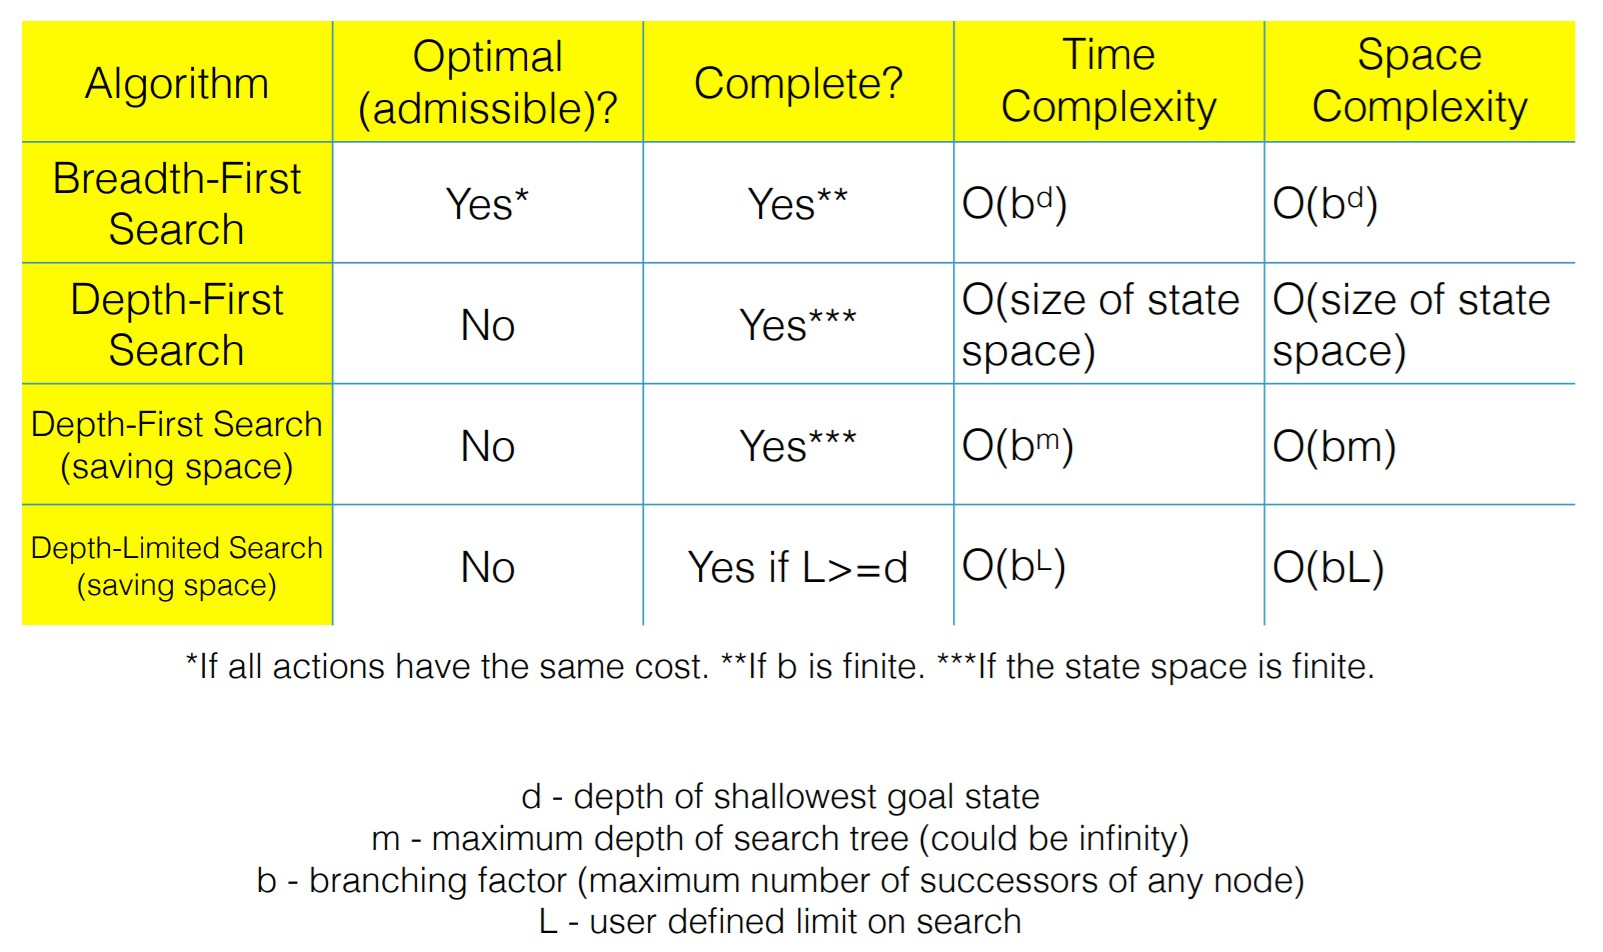
\includegraphics[width=0.8\textwidth]{unit-8/figures/uninformed-search-comparison.jpg}
  \caption*{Comparison of uninformed search algorithms.}
\end{figure}


\section{Informed (Heuristic) Search}
\subsection{Best-First Search}

Breadth-first and depth-first search are examples of the more generic \emph{best-first} search algorithm, in which the frontier node visited next is that with the lowest estimated solution cost, given by an evaluation function \( \function{f}{\text{node}} \).
For breadth-first search, the estimated solution cost of a node is its depth; shallower nodes are visited first.
For depth-first search, the estimated solution cost is the negative of the depth; deeper nodes are visited first.

In order to improve efficiency over uninformed search algorithms, \emph{informed} search algorithms use problem-specific knowledge beyond what is included in the problem formulation.
Commonly, this knowledge takes the form of a \emph{heuristic} function \( \function{h}{\text{node}} \) that maps a node to the estimated cost of the cheapest path from its state to a goal state.
This is used as a guide in order to reduce the number of node expansions required in order to find a goal state.

Since the use of a heuristic function is intended to improve efficiency, it must be simple and quick to compute.
Thus, heuristics are approximate and not guaranteed to work.
For example, in the problem of finding a route between an origin and a destination, following existing paths between cities, a useful heuristic may be the straight-line distance of each city from the destination.
The increase in efficiency over the uninformed search is dependent on the quality of the heuristic.

\subsection{A* Search}

The \emph{A* search} is a popular best-first informed search algorithm that can be used to solve problems in which the costs of actions may differ.
Its evaluation function \( \function{f}{\text{node}} \) is the sum of the costs of the actions taken to reach the current node \( \function{g}{\text{node}} \) and a heuristic function \( \function{h}{\text{node}} \).
\begin{equation*}
  \function{f}{\text{node}} = \function{g}{\text{node}} + \function{h}{\text{node}}
\end{equation*}

To perform an A* search
\begin{enumerate}
  \item visit the frontier node with the smallest \( \function{f}{\text{node}} \) first, placing its children in the frontier, but
  \item do not place a child in the frontier if its corresponding state is represented by a node already in the list of visited nodes, and
  \item if the state of a child is represented by a node already in the frontier, and the node already in the frontier has a larger \( \function{g}{\text{node}} \), remove it and add the new child node to the frontier.
  \item Stop searching when a goal node is visited.
\end{enumerate}

In order to find the optimal solution, it is necessary that the search only terminates in success when a goal node is visited.

A heuristic is \emph{consistent} if the heuristic cost from any node to a goal node is less than or equal to the sum of the actual cost from the node to any other node and the heuristic cost from that node to the goal.
Thus, a consistent heuristic gives an underestimate rather than an overestimate.
\begin{equation*}
  \function{h}{n} \leq \function{\text{cost}}{n, n'} + \function{h}{n'}
\end{equation*}

\begin{figure}[htp]
  \centering
  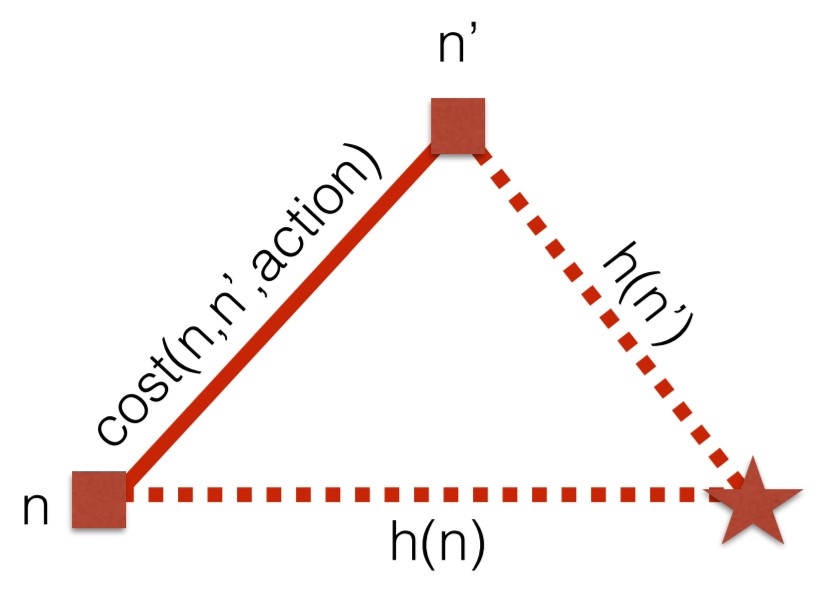
\includegraphics[width=0.3\textwidth]{unit-9/figures/heuristic-consistency.jpg}
  \caption*{The consistency of a heuristic.}
\end{figure}

An A* search has the following properties.
\begin{itemize}
  \item It is complete for any consistent heuristic --- if the heuristic is consistent, the search is guaranteed to find a path to a goal state if one exists, or to terminate in failure otherwise.
  \item It is optimal for any consistent heuristic --- if the heuristic is consistent, the search is guaranteed to find the shortest path to a goal state.
  \item It is optimally efficient for any consistent heuristic --- no other optimal search algorithm using the same heuristic is guaranteed to expand fewer nodes.
\end{itemize}

The time and space complexities of the A* search depend on the state space.
Usually, they are exponential in the depth \( d \) of the optimal solution and in the relative error \( e \) of the heuristic (\( \function{O}{b^{ed}} \)).
\begin{equation*}
  e = \frac{\text{actual cost} - \text{heuristic cost}}{\text{actual cost}}
\end{equation*}
A good heuristic is able to reduce space and time complexity considerably in comparison to an uninformed search.
A heuristic that has a small relative error \( e \), or that can effectively reduce the branch factor \( b \) close to one, will produce very large savings.

In order to improve efficiency, a heuristic can be designed that is more accurate, but not strictly consistent.
In this case, it may be possible to find a good solution without expanding as many nodes, but the solution is not guaranteed to be optimal.

One disadvantage of A* search is that heuristics are problem-specific and can be difficult to devise.
A good idea is to base the heuristic on a relaxed version of the problem --- one with fewer restrictions on actions.
For example, a relaxed version of the sliding tile puzzle may allow tiles to move over other tiles.
A possible heuristic for a state of the puzzle  is the sum of the Manhattan distances between each tile and its goal position.

The A* search algorithm can be applied to any graph-traversal problem.
It is often used for path-finding in video games.


\section{Optimisation}
\subsection{Search and Optimisation}

A search algorithm systematically explores a search space, keeping a tree that represents possible paths, and returns a path to a goal, which describes the solution as a sequence of actions.
When the sequence of actions is not important, and only a near optimal solution is required, it is possible to use algorithms that are more space efficient and do not require complex heuristics.

\emph{Optimisation problems} are solved by finding a solution that minimises or maximises an \emph{objective function}.
A problem may have \emph{constraints} that a solution must satisfy in order to be feasible.
Common optimisation problems include routing, bin packing, scheduling and hyperparameter optimisation.

Unlike a search algorithm, an \emph{optimisation algorithm} does not find a solution by building a path from an initial state to a goal state.
Instead, it maintains an entire \emph{candidate solution}, which may or may not be feasible, and modifies it until it is optimal or near optimal.

Since many search problems have costs associated to actions, they can be formulated as optimisation problems.
Similarly, optimisation problems can often be formulated as search problems with cost functions.
Optimisation algorithms can be used to solve search problems if a suitable objective function can be derived.

The advantages of optimisation algorithms over search algorithms are that
\begin{itemize}
  \item they are usually more space efficient, since
  \begin{itemize}
    \item they do not maintain paths to solutions,
    \item they usually require a fixed amount of space throughout the optimisation process, and
    \item they are usually able to find reasonable solutions to problems with a large state space, for which tree-based search algorithms are unsuitable,
  \end{itemize}
  \item they can sometimes be more time efficient, depending on the algorithm used, and
  \item they do not necessarily require problem-specific heurisitics.
\end{itemize}

Their disadvantages are that
\begin{itemize}
  \item although they can often find a good solution in a reasonable amount of time, they are not guaranteed to retrieve the optimal solution in a reasonable amount of time, and
  \item they are not guaranteed to be complete (they are not guaranteed to find a feasible solution) --- this depends on the problem formulation and operators.
\end{itemize}

\subsection{Learning and Optimisation}

Machine learning can be seen as a problem of finding parameters that minimise a loss function over all possible examples, including unseen data.
It is impossible to calculate the loss of a model on unseen data during training.
Thus, machine learning can be seen as a problem of optimising an objective function that cannot be computed.

Optimisation is a problem of minimising or maximising the value of a known objective function.
Nevertheless, there exist optimisation problems for which the exact value of the objective function cannot be computed.
Some optimisation algorithms can be used as machine learning algorithms that minimise a loss function over training data.

\subsection{Problem Formulation}

The general formulation of an optimisation problem is to minimise some objective functions
\begin{equation*}
  \function[_{k}]{f}{\boldsymbol{x}}, \quad k = 1, \ldots, p
\end{equation*}
subject to some constraints
\begin{gather*}
  \function[_{i}]{g}{\boldsymbol{x}} \leq 0, \quad i = 1, \ldots, m \\
  \function[_{j}]{h}{\boldsymbol{x}} = 0, \quad j = 1, \ldots, n
\end{gather*}

The \emph{design variable} \( \boldsymbol{x} \) is a representation of a candidate solution.
The search space comprises all possible values of the design variable.
A candidate solution replaces the initial state and goal state required for the formulation of a search problem.

An objective function defines a quality to be maximised or a cost to be minimised.
All maximisation problems can be formulated as minimisation problems and vice versa.
An optimisation problem with multiple objective functions is known as a \emph{multi-objective} optimisation problem.
The objective functions replace the cost function required for the formulation of a search problem.

An optimisation problem may define constraints that a solution must satisfy in order to be feasible.
The constraints replace the list of possible actions and their effects required for the formulation of a search problem.
All constraints can be represented in the form of the inequality constraint \( \function[_{i}]{g}{\boldsymbol{x}} \leq 0 \) or the equality constraint \( \function[_{j}]{h}{\boldsymbol{x}} = 0 \).

For example, the problem formulation for minimising the distance travelled on a route between an origin city and a destination city, using only defined paths between neighbouring cities on a given a map of \( N \) cities, is as follows.

Minimise the objective function
\begin{equation*}
  \function{f}{\boldsymbol{x}} = \sum_{i=1}^{\left\lvert \boldsymbol{x} \right\rvert - 1} D_{x_{i},x_{i+1}}
\end{equation*}
subject to the constraints
\begin{gather*}
  \function[_{1}]{h}{\boldsymbol{x}} = 0 \\
  \function[_{2}]{h}{\boldsymbol{x}} = 0
\end{gather*}
where
\begin{itemize}
  \item \( \boldsymbol{x} \) has any size, and its elements \( x_{i} \in \left\{ 1, \ldots, N \right\} \) each represent one of the \( N \) cities,
  \item \( \mathbf{D} \) is a matrix of distances, with each element \( D_{i,j} \) being the distance to travel along the single path from city~\( i \) to its direct neighbour city~\( j \), or \( -1 \) if such a path does not exist,
  \item the constraint to ensure that each step of the route is a defined path between two neighbouring cities is defined by
  \begin{equation*}
    \function[_{1}]{h}{\boldsymbol{x}} = \begin{cases}
      0 & \text{if } D_{x_{i},x_{i+1}} \not= -1, \quad \forall i \in \left\{ 1, \ldots, \left\lvert \boldsymbol{x} \right\rvert - 1 \right\} \\
      1 & \text{otherwise}
    \end{cases}
  \end{equation*}
  \item the constraint to ensure that the route begins at the origin city \( 1 \) and ends at the destination city \( N \) is defined by
  \begin{equation*}
    \function[_{2}]{h}{\boldsymbol{x}} = \begin{cases}
      0 & \text{if } x_{1} = 1 \text{ and } x_{\left\lvert \boldsymbol{x} \right\rvert} = N \\
      1 & \text{otherwise}
    \end{cases}
  \end{equation*}
\end{itemize}

\subsection{Hill Climbing}

Assuming maximisation, the \emph{hill~climbing} algorithm operates as follows.
\begin{enumerate}
  \item Initialise the current solution by generating an initial candidate solution at random.
  \item Repeating until the maximum number of iterations is reached,
  \begin{enumerate}
    \item generate neighbour solutions --- candidate solutions that differ from the current solution by a single element,
    \item get the best neighbour solution --- the neighbour solution with the greatest quality.
    \item If the quality of the best neighbour is less than or equal to the quality of the current solution, do not change the current solution.
    \item Otherwise, replace the current solution with the best neighbour solution.
  \end{enumerate}
\end{enumerate}

The advantage of hill~climbing is that it very quickly finds the nearest solution of optimal quality.
However, this solution may be a local optimum rather than the global optimum.
This is because it is a \emph{greedy} algorithm --- it does not accept neighbours of equal or worse quality, only better.
For the same reason, the current solution may become trapped on a plateaux --- a series of neighbour solutions with equal quality.
The success of the algorithm depends on the shape of the objective function.
As the algorithm is relatively simple, it can be used before more complex algorithms are investigated.

Hill~climbing has the following properties.
\begin{itemize}
  \item It is not guaranteed to be optimal.
  \item Its worst-case time complexity, assuming a maximum number of iterations \( m \), a maximum number of neighbours generated per iteration \( n \) and that the generation of neighbours has time complexity \( \function{O}{p} \), is \( \function{O}{mnp} \).
  \item Its worst-case space complexity, assuming a maximum number of neighbours generated per iteration \( n \) and that the design variable has space complexity \( \function{O}{q} \), is \( \function{O}{nq} \).
\end{itemize}

The completeness of the algorithm --- whether is is guaranteed to find a feasible solution --- depends on the problem formulation and operators.

\subsection{Simulated Annealing}

In the \emph{simulated~annealing} algorithm, it is a random neighbour, rather than the best neighbour, that is compared to the current solution.
There is also a probability-based chance for the current solution to be replaced by a worse neighbour on each iteration.

The probability of accepting a solution of equal or worse quality (or a solution of equal or greater cost) than the current solution is inspired by thermodynamics, giving the algorithm its name.
It is defined in terms of an \emph{error} \( \Delta E \) --- the difference between the qualities of the random neighbour and the current solution --- and a \emph{temperature} \( T \).
\begin{equation*}
  e^{\frac{\Delta E}{T}}, \quad \Delta E \leq 0, \quad T > 0
\end{equation*}
Since the probability is only used when the random solution is of equal or worse quality to the current solution, the error is always less than or equal to zero.
Additionally, the temperature is defined to be always greater than zero.
Thus, the probability decreases from one and approaches zero asymptotically as the error increases in magnitude (decreases further below zero) and the temperature decreases.

The temperature \( T \) is set to a high initial value (a parameter of the algorithm).
It is gradually reduced by update rules or \emph{schedules} as the algorithm progresses.
Typically, it is multiplied by a positive coefficient close to and smaller than one on each iteration.
\begin{equation*}
  \text{Let } T = \alpha T, \quad \alpha = 0.95
\end{equation*}
This ensures that the temperature remains above zero and decreases slowly enough for the algorithm to explore the search space and pass over small optima.

Thus, when used in the simulated~annealing algorithm, the probability for the random neighbour to replace the current solution has the following properties.
\begin{itemize}
  \item It decreases as the quality of the random neighbour decreases.
  This ensures that the current solution does not stray too far from an optimum.
  \item It decreases slowly as the algorithm progresses.
  This increases the basis of attraction over time, and allows smaller optima in the search space to be passed without exploitation initially.
\end{itemize}

Assuming maximisation, the \emph{simulated~annealing} algorithm, with the input parameters of initial temperature and minimum temperature, operates as follows.
\begin{enumerate}
  \item Initialise the current solution by generating an initial candidate solution at random.
  \item Set the temperature to the initial temperature.
  \item Repeating until the minimum temperature is reached, or the current solution stops changing,
  \begin{enumerate}
    \item generate a random neighbour solution --- a candidate solution that differs from the current solution by a single element.
    \item If the quality of the random neighbour is less than or equal to the quality of the current solution, decide based on the probability \( e^{\frac{\Delta E}{T}} \) whether to replace the current solution with the random neighbour solution.
    \item Otherwise, replace the current solution with the random neighbour solution.
    \item Update (schedule) the temperature.
  \end{enumerate}
\end{enumerate}

Simulated~annealing is also a local search algorithm, as it only allows the current solution to move between neighbours.
It employs methods to escape from local optima, however.
The algorithm has the following properties.
\begin{itemize}
  \item It is not guaranteed to find the optimal solution in a reasonable amount of time.
  \item Its time complexity is difficult to compute, as it depends on the schedule, minimum temperature and properties of the problem formulation.
  \item Its space complexity depends on the representation of the design variable.
\end{itemize}

The completeness of the algorithm --- whether is is guaranteed to find a feasible solution --- depends on the problem formulation and operators.

Whether it finds the optimal solution depends on the schedule and minimum temperature.
If left to run indefinitely with a relaxed schedule, it is guaranteed to find the optimal solution, but this may take longer than the time needed to enumerate all possible solutions using brute force.
Therefore, the advantage of simulated~annealing is that it can frequently obtain near optimal solutions by escaping from poor local optima in a reasonable amount of time.

\subsection{Handling Constraints}

\subsubsection{Travelling Salesman Problem (TSP)}

In the \emph{travelling salesman problem} (TSP), a salesman must travel through \( N \) cities, subject to the following constraints.
\begin{itemize}
  \item Each city must be visited once and only once (an explicit constraint).
  \item The salesman must begin and end the journey at the same city (an implicit constraint of the objective function).
  \item Only the \( N \) cities may appear on the route (an implicit constraint of the design variable).
\end{itemize}
Each pair of cities has a distance between them.
The total distance of the solution route is to be minimised.

The problem formulation is as follows.

Minimise the objective function
\begin{equation*}
  \function{f}{\boldsymbol{x}} = \left( \sum_{i=1}^{N-1} D_{x_{i},x_{i+1}} \right) + D_{x_{N},x_{1}}
\end{equation*}
subject to the constraint
\begin{equation*}
  \function[_{i}]{h}{\boldsymbol{x}} = 0, \quad \forall i \in \left\{ 1, \ldots, N \right\}
\end{equation*}
where
\begin{itemize}
  \item \( \boldsymbol{x} \) is a sequence of \( N \) cities, and its elements \( x_{i} \in \left\{ 1, \ldots, N \right\} \) each represent one of the \( N \) cities,
  \item \( \mathbf{D} \) is a matrix of distances, with each element \( D_{i,j} \) being the distance to travel along the single path from city~\( i \) to its direct neighbour city~\( j \),
  \item the constraint to ensure that a city \( i \) appears once and only once in the route is defined by
  \begin{equation*}
    \function[_{i}]{h}{\boldsymbol{x}} = \left( \sum_{j=1}^{N} 1 \left( x_{j} = i \right) \right) -1 = 0
  \end{equation*}
  using the \emph{indicator} function
  \begin{equation*}
    1 \left( x_{j} = i \right) \begin{cases}
      1 & \text{if } x_{j} = i \\
      0 & \text{if } x_{j} \not= i
    \end{cases}
  \end{equation*}
\end{itemize}

\subsubsection{Representation, Initialisation and Neighbourhood Operators}

Most real-world problems have constraints.
Optimisation algorithms do not usually include strategies for dealing with constraints.
Instead, strategies must be designed for each problem.
One way of doing this is to design the solution representation, initialisation and neighbourhood operators in such a way that they ensure the constraints are always satisfied.

The representation for a TSP solution could be an array of size \( N \), where \( N \) is the number of cities to visit.
The omission from the representation of the return to the origin city helps to deal with the implicit constraint that the salesman must begin and end the journey at the same city.

The initialisation method for a TSP solution could be to draw cities uniformly at random from the set \( \left\{ 1, \ldots, N \right\} \) without replacement.
This ensures that no cities are missing or duplicated in the initial solution (an explicit constraint), and that only the cities in the given set are visited (an implicit constraint).

The neighbourhood operator for a TSP solution could reverse the path between two randomly selected cities.
Alongside the initialisation method, this ensures that no cities are missing or duplicated in neighbourhood solution (an explicit constraint), and that only the cities in the given set are visited (an implicit constraint).

Together, this design of representation, initialisation and neighbourhood operator ensures that the constraints of the problem are satisfied.

The advantage of handling constraints in this way is that it is ensured that no infeasible candidate solutions are generated.
However, the design is problem-specific, and may be difficult to derive.
Additionally, it may restrict the search space too harshly, making it difficult to find the optimal solution.

Using this strategy, optimisation algorithms such as hill~climbing and simulated~annealing are complete, as infeasible solutions are never generated.

\subsubsection{Objective Function}

Another method of handling constraints is to modify the objective function such that it penalises any infeasible solution by increasing its cost.

For example, assuming the representation for a TSP solution is a list of cities of any size, and that the initialisation method allows missing and duplicate cities, two properties of a candidate solution would be the number of missing cities \( n_{\mathrm{m}} \) and the number of duplicate cities \( n_{\mathrm{d}} \).
These could be multiplied by a large positive constant \( P \) and included as penalty terms in the objective function.
\begin{equation*}
  \function{f}{\boldsymbol{x}} = \left( \sum_{i=1}^{N-1} D_{x_{i},x_{i+1}} \right) + D_{x_{N},x_{1}} + n_{\mathrm{m}} P + n_{\mathrm{d}} P
\end{equation*}
The value of \( P \) should be large enough such that any infeasible solution is more expensive than any feasible solution.

More generally, the problem formulation is modified as follows.

Minimise the objective functions
\begin{equation*}
  \function[_{k}]{f}{\boldsymbol{x}} + \function{Q}{\boldsymbol{x}}, \quad k = 1, \ldots, p
\end{equation*}
subject to some constraints
\begin{gather*}
  \function[_{i}]{g}{\boldsymbol{x}} \leq 0, \quad i = 1, \ldots, m \\
  \function[_{j}]{h}{\boldsymbol{x}} = 0, \quad j = 1, \ldots, n
\end{gather*}
where the penalty function \( \function{Q}{\boldsymbol{x}} \) is zero if the solution is feasible, or the weighted sum of the squares of only the violated constraints otherwise.
\begin{equation*}
  \function{Q}{\boldsymbol{x}} = \begin{cases}
    0 & \text{if } \boldsymbol{x} \text{ is feasible} \\
    P \left( \function[_{a}]{g}{\boldsymbol{x}}^{2} + \function[_{b}]{g}{\boldsymbol{x}}^{2} + \ldots + \function[_{a'}]{h}{\boldsymbol{x}}^{2} + \function[_{b'}]{h}{\boldsymbol{x}}^{2} + \ldots \right) & \text{ otherwise}
  \end{cases}
\end{equation*}

Only the constraints that are violated are included in the penalty.
This ensures that unviolated inequality constraints do not penalise the solution.
The values of the constraints are squared to ensure they are positive and increase the cost of the solution.

The advantage of handling constraints in this way is that the penalty is general and could be applied to any optimisation problem.
However, the algorithm must search for feasible solutions amongst infeasible solutions.
This may be a poor choice of strategy for problems in which there are many infeasible solutions.

Using this strategy, optimisation algorithms such as hill~climbing and simulated~annealing may not be complete, as infeasible solutions may be generated.
In particular, hill~climbing is not complete if the object function has local optima, and simulated~annealing is not guaranteed to find a feasible solution within a reasonable amount of time.


\section{Evolutionary Algorithms}
\subsection{Background}

\emph{DNA} is a chemical compound that contains the instructions for developing a living organism.
A \emph{gene} is a region of DNA that influences a particular characteristic of an individual.
An \emph{allele} is one possible form of a particular gene.
A \emph{chromosome} is a structure that holds a molecule of DNA\@.
The \emph{genotype} of an individual is its complete set of DNA, whereas its \emph{phenotype} is its observed characteristics.

\emph{Evolution} is the change in inherited traits of a population of organisms through successive generations.
This occurs when there is a change in the frequency of certain alleles in a population over time.
Evolution is caused by \emph{genetic variation} and \emph{natural selection}.

Genetic variation is caused by sexual reproduction, which can introduce new combinations of genes into a population, and mutation, which is a natural process that alters the DNA sequence of an individual, allowing variations that are not present in its parents.

Natural selection is the differential survival and reproduction of individuals due to differences in phenotype.
Some phenotypes may protect individuals from prey, or increase the likelihood of attracting mates, thereby increasing the chance of survival and reproduction.
Genotypes that are more likely to leave offspring are known as \emph{fitter} genotypes.
A genotype that is fit for one environment may not be fit for another.

In the case of an evolutionary algorithm, a fitter solution is one that has higher quality in terms of the objective function, and is, therefore, more likely to be used in the generation of new solutions.
After many iterations, solutions improve with respect to the objective function.

\subsection{Behaviour of an Evolutionary Algorithm}

In a population of candidate solutions, parent solutions are selected, recombined and mutated to produce offspring solutions.
Survivors are selected from the population for the next iteration.
The selection of parents and survivors is based on selective pressure towards fitter solutions.
There is a small chance that poor individuals survive to the next iteration.
Over many iterations, the population of solutions becomes more optimal.

Hill~climbing is a greedy local search algorithm that climbs from an initial solution to the nearest optimum.
Its solution can become trapped at a local optimum or a plateau.
Simulated~annealing is also a non-greedy local search algorithm.
It gives some probability towards accepting a worse solution.
The probability is initially high to allow exploration of the search space.
It decreases gradually to allow promising optima to be exploited.

Evolutionary algorithms maintain a population of candidate solutions rather than a single solution.
This helps to explore different regions of the search space.
The small probability of poor solutions being selected for recombination and survival helps to avoid local optima.
Evolutionary algorithms are global search algorithms.
They can generate new solutions that are not neighbours of current solutions.
One disadvantage of this is that some optima may not be visited.

\begin{figure}[!htp]
  \centering
  \caption*{Typical behaviour of an evolutionary algorithm.}
  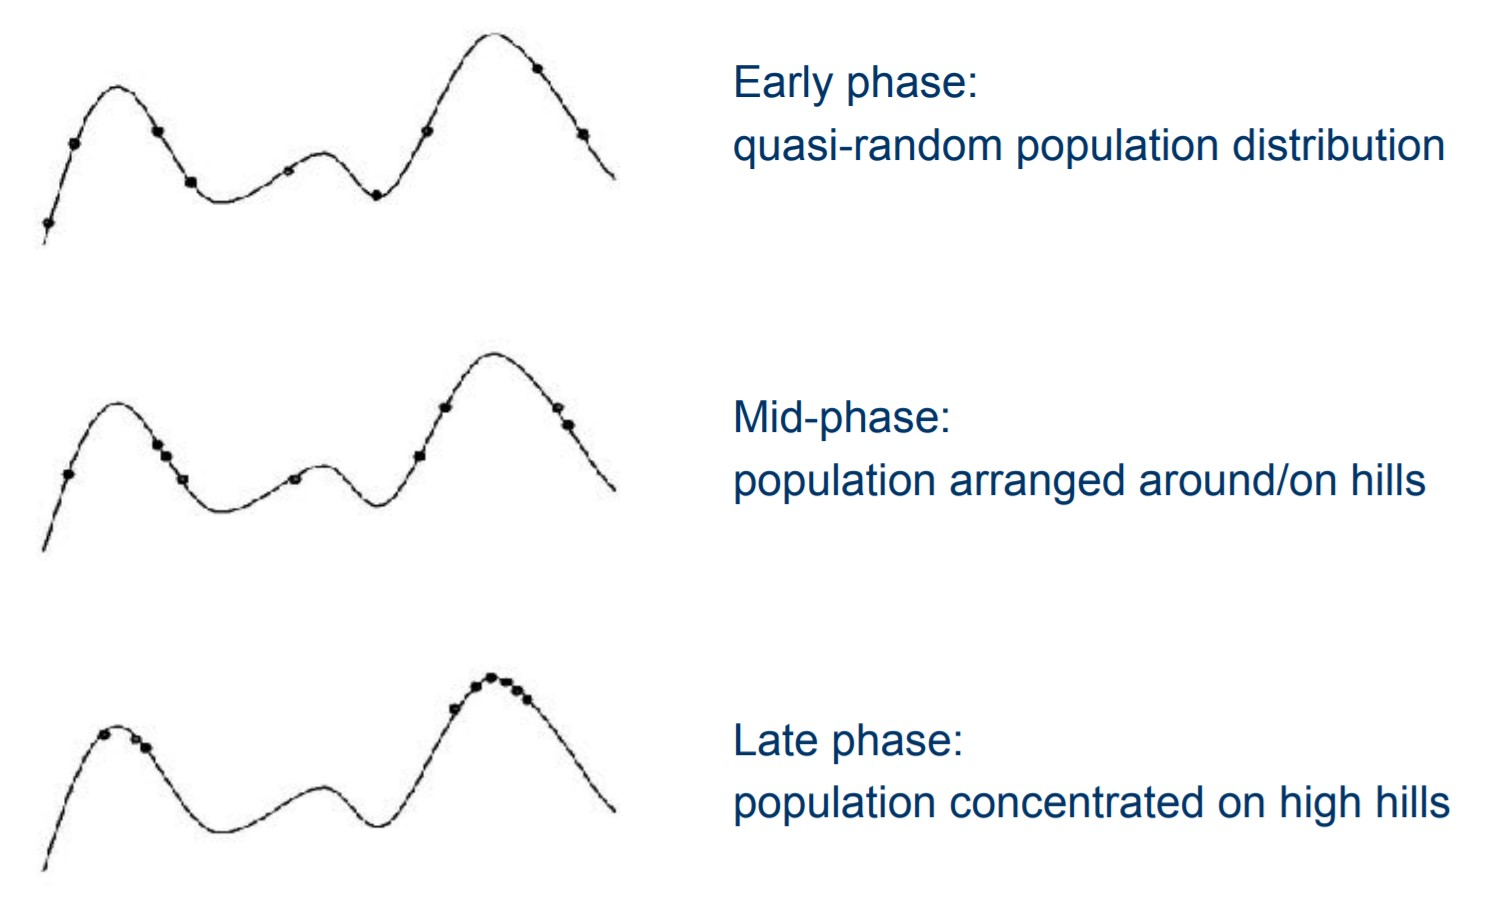
\includegraphics[width=0.6\textwidth]{unit-11/figures/phases.jpg}
\end{figure}

An evolutionary algorithm proceeds as follows.
\begin{enumerate}
  \item Initialise the population
  \item Evaluate the fitness of each solution
  \item Repeat until a termination condition is satisfied
  \begin{enumerate}
    \item Select parent solutions
    \item Recombine parent solutions with a probability \( P_{\mathrm{c}} \)
    \item Mutate resulting offspring with a probability \( P_{\mathrm{m}} \)
    \item Evaluate the fitness of each offspring solution
    \item Select survivors for the next iteration
  \end{enumerate}
\end{enumerate}
The selection of parents and survivors is based on selective pressure towards fitter solutions.

\subsection{Representation}

The representation of a candidate solution is its \emph{genotype} or \emph{encoding}.
The value of a solution is its \emph{phenotype}.
A phenotype that cannot be represented in the genotypic space cannot exist.
A representation must allow all feasible solutions to be represented.
It is useful for the representation to be easily manipulated by the algorithm.

Traditionally, a candidate solution for an evolutionary algorithm is represented as a \emph{binary~vector} or \emph{binary~string}.
Each position in the vector can assume a value of zero or one.
The genotypic space \( \left\{ 0, 1 \right\}^{L} \) is a binary~vector of length \( L \)\@.
Each position in the vector is a \emph{gene}.
The value of a gene is an \emph{allele}.

Integer vectors are useful for discrete, ordinal or categorical problems, floating-point vectors are useful for continuous problems, and matrices are useful for multidimensional problems such as staff allocation.

To \emph{encode} is to create a representation for a particular candidate solution.
To \emph{decode} is to recover the candidate solution from its representation.

It may be possible to encode a particular solution in more than one way using the representation, in which case, not all phenotypes would have the same chance of appearing in the initial population.
Nevertheless, a genotype or representation must decode to only one phenotype or candidate solution.

\subsection{Initialisation}

Initialisation is usually performed at random to ensure an even distribution of possible alleles.
One method of random initialisation is to initialise individual genes uniformly at random.
The initialisation process can make use of existing solutions or problem-specific heuristics to seed the population.
This increases the probability of generating initial solutions in regions that are more promising.

\subsection{Evaluation}

A \emph{fitness~function} assigns a value of fitness to each phenotype, and represents the requirements to which the population should adapt.
Often, the objective function is used as the fitness function.
The function may include strategies for dealing with constraints.
Typically, an evolutionary problem is formulated in terms of maximising fitness.
All minimisation problems can be formulated as maximisation problems.

\subsection{Parent Selection}

The selection of parent solutions is usually based on a probability such that
\begin{itemize}
  \item fitter solutions are more likely to be selected, and
  \item even the worst solutions have some chance of being selected.
\end{itemize}
The stochastic nature of parent selection helps to avoid solutions becoming trapped at local optima.

The number of parents to select is a design choice of the algorithm.
Commonly, the number of parents is chosen such that the number of offspring is equal to the current size of the population.
Two methods of parent selection are \emph{roulette wheel} and \emph{tournament} selection.

In roulette wheel selection, the probability of selection for an individual solution is proportional to its fitness.
The probability of selection for a solution \( a \), given a fitness function \( \function{f}{x} \) and that all solutions \( x \) belong to the current population \( X \), is given by
\begin{equation*}
  \frac{\function{f}{a}}{\sum_{x \in X} \function{f}{x}}
\end{equation*}
Since a parent must be selected from the current population, the probabilities for each candidate solution sum to one.

Disadvantages of roulette wheel selection are that
\begin{itemize}
  \item individual solutions of outstanding fitness may take over the population very quickly, causing \emph{premature convergence},
  \item when solutions have similar fitness, there is very little \emph{selective pressure}, and
  \item the mechanism behaves differently for transpositions of the fitness function that should result in the same solution.
\end{itemize}

In tournament selection, \( k \) solutions are picked from the population uniformly at random.
The selected parent is the fittest of these solutions.
This process is repeated to select more parents.
Tournament selection is able to apply selective pressure even when parents have similar fitness.

\subsection{Recombination}

Recombination is a process that generates offspring solutions based on parent solutions.
Recombination involving two parents is known as \emph{crossover}.
The recombination probability \( P_{\mathrm{c}} \) determines whether recombination occurs.
If it does not occur, the parents are cloned.
Most offspring will be similar or worse than their parents due to the random selection of parent genes.
Some offspring will be fitter, however.
\emph{Genetic algorithms} are evolutionary algorithms that have a high recombination probability, typically in the interval \( \left[ 0.6, 0.9 \right] \).

In \emph{single-point crossover}, a point between two positions in a representation vector is selected at random.
The parent solutions are split at the point, and their tails are exchanged.
The resulting crossovers are the children.

Single-point crossover has a number of disadvantages that arise from positional bias.
Its performance depends on the order that components of the design variable occur in the representation.
Adjacent genes are more likely to be kept together, and two genes from opposite ends of the vector can never be kept together.
This bias can be exploited if knowledge of the structure of the problem suggests that some genes should be kept together.

\emph{Multi-parent recombination} produces offspring from multiple parents using \emph{diagonal crossover}.
For \( k \) parents, \( k - 1 \) splitting points are selected.
Children are created from the split sections of their parents along diagonals.

\begin{table}[!htp]
  \centering
  \caption*{Diagonal crossover of three parents, each split into three sections A, B and C.}
  \begin{tabular}{ccccccc}
    \toprule
    \multicolumn{3}{c}{Parents} & & \multicolumn{3}{c}{Offspring} \\
    \midrule
    \textcolor{red}{A\textsubscript{1}} & \textcolor{blue}{B\textsubscript{1}} & \textcolor{green}{C\textsubscript{1}} & &
    \textcolor{red}{A\textsubscript{1}} & \textcolor{red}{B\textsubscript{2}} & \textcolor{red}{C\textsubscript{3}} \\
    \textcolor{green}{A\textsubscript{2}} & \textcolor{red}{B\textsubscript{2}} & \textcolor{blue}{C\textsubscript{2}} & &
    \textcolor{green}{A\textsubscript{2}} & \textcolor{green}{B\textsubscript{3}} & \textcolor{green}{C\textsubscript{1}} \\
    \textcolor{blue}{A\textsubscript{3}} & \textcolor{green}{B\textsubscript{3}} & \textcolor{red}{C\textsubscript{3}} & &
    \textcolor{blue}{A\textsubscript{3}} & \textcolor{blue}{B\textsubscript{1}} & \textcolor{blue}{C\textsubscript{2}} \\
    \bottomrule
  \end{tabular}
\end{table}

\emph{Intermediate recombination} for floating-point representations produces an offspring from the simple average of its parents.

\subsection{Mutation}

Mutation acts on one genotype and produces another.
This typically causes small changes to the solution.
It can introduce traits that did not originally exist in the population.

For binary vector representations, \emph{bitwise bit-flipping} is used.
Each gene (bit) is flipped with the probability \( P_{\mathrm{m}} \), which is known as the \emph{mutation rate}, and is typically in the interval
\begin{equation*}
  \left[ \frac{1}{\text{population size}}, \frac{1}{\text{genotype length}} \right]
\end{equation*}

For integer representations, \emph{random reset} or \emph{creep mutation} are used.
Random reset is most suitable for categorical design variables.
A new value is selected from the set of permissible values (excluding the current value) according to a discrete uniform distribution.
This means that each value has the same probability of selection.
Creep mutation is most suitable for ordinal design variables.
A new value is selected from the set of permissible values (excluding the current value) according to a discrete non-uniform distribution centred around the current value.
This can be achieved by adding a value from a binomial distribution to the current value and subtracting the mean of the distribution.

Uniform mutation for a floating-point representation is similar to a random reset.
A new value is selected from a continuous uniform distribution.
This means that each possible value has the same probability of selection.
Non-uniform mutation for a floating-point representation is similar to creep mutation.
The new value is generated using a continuous non-uniform distribution, such as a normal distribution.
This means that smaller changes are more likely than larger changes, and that an increase by a certain amount is equally as likely as a decrease by the same amount.

\subsection{Survival Selection}

Typically, solutions are selected for survival such that the population maintains a constant size.
The two main types of survival selection are \emph{age-based} and \emph{fitness-based}.

In age-based survival selection, all offspring solutions survive, and the previous generation dies.
The problem with this method is that fit solutions from the previous generation are lost.

One type of fitness-based survival selection is \emph{delete-worst} selection.
This removes the worst solutions from both the offspring and the previous generation, ensuring only the best solutions survive.
The problem with this method is that it can result in premature convergence.

Another type of fitness-based survival selection is \emph{elitism}, which is usually combined with age-based selection.
In general, all offspring survive, but if the offspring generation does not contain the best solution, the worst child is replaced by the best solution from the previous generation.

\subsection{Termination}

Commonly, the algorithm is terminated when
\begin{itemize}
  \item a maximum number of iterations is reached,
  \item a specified level of fitness is reached,
  \item a minimum level of diversity is reached, or
  \item a maximum number of iterations is reached without any improvement in fitness.
\end{itemize}

\subsection{Summary}

Evolutionary algorithms can be applied to a variety of optimisation problems.
Thus, it can be said that evolutionary algorithms are \emph{problem independent}.
Nevertheless, the choice of fitness function, constraint strategy, representation, initialisation, parent selection, recombination, mutation, survival selection and termination criteria depends on the problem.

\begin{description}
  \item[population] a multiset of individuals
  \item[individual] a candidate solution
  \item[genotype] the representation of a candidate solution
  \item[chromosome] the representation of a candidate solution
  \item[gene] a component of a chromosome
  \item[allele] the value of a gene
  \item[mutation] a unary variation operator that generates a new individual
  \item[crossover] a binary variation operator that generates one or more new individuals
  \item[recombination] an \( n \)-ary variation operator that generates one or more new individuals
  \item[fitness function] a function to be optimised by the evolutionary algorithm
  \item[generation] iteration
\end{description}


\section{Reinforcement Learning}
\subsection{Concepts}

\subsubsection{Sparse Data}

\emph{Reinforcement learning} is a process by which an agent learns to interact with an environment based on the feedback signals (rewards) it receives from the environment, in order to achieve a goal efficiently.
Unlike supervised learning, reinforcement learning does not require any background knowledge of the problem or any labelled data.
The agent gains sparse data and time-delayed rewards by interacting with the environment without supervision, rather than learning the structure of training data.
The data gained is sparse because some actions may not result in a reward.
The goal of the agent is to maximise its future rewards, rather than to find a function that maps input to output.

Some advantages of reinforcement learning are that
\begin{itemize}
  \item no human needs to generate training data, and
  \item the performance of the agent is not limited to the performance shown in training data; the agent is permitted to improve by generating new data.
\end{itemize}

\subsubsection{Rewards}

A reward \( R_{t} \) is an immediate feedback signal that indicates the performance of the agent at step~\( t \).
The goal of the agent is to maximise its cumulative reward.
It is not sufficient to maximise the immediate or final rewards, since it is necessary to find the most efficient way to complete the task.
An action may result in a delayed reward, and it may be better to sacrifice an immediate reward for a long-term reward.

\subsubsection{Agent, Environment and State}

At each step \( t \),
\begin{itemize}
  \item the agent
  \begin{itemize}
    \item receives an observation \( O_{t} \),
    \item receives a reward \( R_{t} \), and
    \item executes an action \( A_{t} \),
  \end{itemize}
  \item the environment
  \begin{itemize}
    \item receives the action \( A_{t} \),
    \item emits an observation \( O_{t+1} \), and
    \item emits a reward \( R_{t+1} \), and
  \end{itemize}
  \item the state \( S_{t} \) is a summary of the environment that is used to determine the next action.
\end{itemize}

The agent observes the environment indirectly.
This is known as \emph{partial observation}.
An \emph{episode} is a series of consecutive states that form a single attempt of the agent to complete the task.

\subsubsection{Policy}

The \emph{policy} \( \pi \) of an agent is a function that maps a state \( s \) to an action \( a \).
A \emph{deterministic} policy \( \pi\!\left(s\right) \) always maps a given state to the same action.
\begin{equation*}
  a = \pi\!\left(s\right)
\end{equation*}
A \emph{stochastic} policy \( \pi\!\left(a \vert s \right) \) maps a state to one of many actions based on a probability.
\begin{equation*}
  \pi\!\left(a \vert s \right) = P\!\left( A = a \vert S = s \right)
\end{equation*}
This allows the agent to explore more states and make more observations.

\subsubsection{Value Function}

The \emph{value~function} \( V_{\pi}\!\left(s\right) \) of a state \( s_{t} \) using policy \( \pi \) is a prediction of the future reward that will be received following a transition to that state.
This is used to evaluate the quality of a state.
\begin{equation*}
  V_{\pi}\!\left(s_{t}\right) = E_{\pi}\!\left( R_{t} + \gamma R_{t+1} + \gamma^{2} R_{t+2} \ldots \vert S_{t} = s \right), \quad 0 \leq \gamma \leq 1
\end{equation*}
The \emph{discount~rate} \( \gamma \) reflects the importance of future rewards.
A value of \( \gamma = 0 \) is used to ignore future rewards.
A value of \( \gamma = 1 \) is used to treat immediate and future rewards with the same importance.

\subsubsection{Types of Agent}

A \emph{value-based agent} learns to achieve a task by constructing a value function.
In this case, the policy is implicit and can be derived directly from the value function.

A \emph{policy-based agent} learns to achieve a task by constructing a representation of the policy.
In this case, there is no need for a value function.

An \emph{actor-critic agent} uses both a value function and a policy.

\subsection{\texorpdfstring{\( Q \)}{Q}-Learning}

\emph{\( Q \)-learning} is a model-free and value-based reinforcement learning algorithm.
It learns by constructing an action-value function known as the \emph{\( Q \)-function} that predicts the future reward that will be received following a transition to a state \( s_{t} \) via an action \( a_{t} \).
It is used to evaluate the quality of a state and action pair.
\begin{equation*}
  Q_{\pi}\!\left(s_t, a_{t}\right) = E_{\pi}\!\left( R_{t} + \gamma R_{t+1} + \gamma^{2} R_{t+2} \ldots \vert S = s_{t}, A = a_{t} \right), \quad 0 \leq \gamma \leq 1
\end{equation*}

\( Q \)-learning constructs a matrix known as a \emph{\( Q \)-table} that records the value of the \( Q \)-function for each state and action pair.
This table is used to select the best action at a given state.

The \emph{Bellman~equation} is used to update the \( Q \)-table during the learning process.
The new value \( Q'\!\left( s_{t}, a_{t} \right) \) is calculated using the old value \( Q\!\left( s_{t}, a_{t} \right) \), the \emph{learning~rate} \( \alpha \), the immediate reward \( R\!\left( s_{t}, a_{t} \right) \), the discount~rate \( \gamma \) and the maximum expected future reward \( Q\!\left( s_{t+1}, a \right) \) at state \( s_{t+1} \).
\begin{equation*}
  Q'\!\left( s_{t}, a_{t} \right) = \left( 1 - \alpha \right) Q\!\left( s_{t}, a_{t} \right) + \alpha \left( R\!\left( s_{t}, a_{t} \right) + \gamma \max_{a} Q\!\left( s_{t+1}, a \right) \right)
\end{equation*}

The \( Q \)-learning algorithm proceeds as follows.
\begin{enumerate}
  \item Initialise each element of the \( Q \)-table with the same arbitrary fixed value.
  \item For each episode,
  \begin{enumerate}
    \item select a random initial state, and
    \item until the goal state is reached,
    \begin{enumerate}
      \item select an action at random,
      \item perform the action and move to the corresponding next state,
      \item receive the reward, and
      \item update the entry for the state and action pair in the \( Q \)-table using the Bellman equation.
    \end{enumerate}
  \end{enumerate}
\end{enumerate}

Initially, the \( Q \)-table gives the same arbitrary fixed value for all state and action pairs.
As the states and actions are explored, the \( Q \)-table gives better predictions.

Often, zero is used as the initial value for the \( Q \)-table.
Since \( Q \)-learning is a greedy algorithm, this may lead to the agent always choosing a non-optimal action that has already been explored.
One solution to this problem is to initialise the \( Q \)-table with a high value.
This makes unexplored states and actions more appealing, and encourages the greedy agent to explore.
This is known as \emph{absolute~greedy exploration}.

It is also possible to initialise areas of the \( Q \)-table with different values.
This creates bias towards some states and actions, allowing the agent to take advantage of prior knowledge of the problem.

\subsection{Deep \texorpdfstring{\( Q \)}{Q}-Networks}

For a problem in which there are many states that each have many actions, it is difficult to maintain the \( Q \)-table.
A deep network known as a \emph{deep \( Q \)-network} is used to approximate the \( Q \)-function.
Whereas \( Q \)-learning produces \( Q \)-values for state and action pairs, deep \( Q \)-learning takes a state as an input and produces the \( Q \)-values of each action available at the given state.

\subsection{Policy Gradient}

A value-based algorithm such as \( Q \)-learning cannot handle continuous input or sparse rewards.
It also cannot learn a stochastic policy.
This means that it cannot easily explore the reward space.
These problems are solved by policy-based agents.

\emph{Policy gradient} is a model-free and policy-based reinforcement learning algorithm.
It begins by creating an arbitrarily random policy and exploring for several episodes.
The probabilities of actions that lead to a high reward are increased.
The probabilities of actions that lead to a low reward are decreased.

The quality of a policy \( \pi_{\theta} \) on a network \( \theta \) is measured using a score function \( J\!\left( \theta \right) \) that operates on the stored transitions of all episodes where the agent used the policy \( \pi_{\theta} \), and calculates the probabilities that the environment is in state \( s \) and that the agent takes action \( a \) in that state.
Each stored transition consists of a state \( s \), an action \( a \) and a reward \( R\!\left( s, a \right) \).
\begin{equation*}
  J\!\left( \theta \right) = \sum_{s} \left( P\!\left( s \right) \sum_{a} \left( P\!\left( a \vert s \right) R\!\left( s, a \right) \right) \right)
\end{equation*}
The parameters of the policy are updated via gradient ascent, where the gradient is that of the score of the policy.

\subsection{Model-Free and Model-Based Learning}

Both \( Q \)-learning and policy gradient are \emph{model-free} algorithms.
This means that the agent is given no prior knowledge of the problem.

A \emph{model-based} algorithm uses a model that describes the distribution of states and rewards in the environment.
This allows the agent to make informed decisions and reduces the need to explore.

\subsection{Actor-Critic Learning}

While policy gradient can handle both continuous and discrete action spaces, it takes longer to train than \( Q \)-learning since it needs to collect more data.
An actor-critic agent uses aspects of both value-based and policy-based learning to provide a balance between exploration of the environment and exploitation of reward.

\subsection{\texorpdfstring{\( \varepsilon \)}{Epsilon}-Greedy Exploration}

The \( Q \)-learning algorithm can be modified to provide a balance between exploration and exploitation using \emph{\( \varepsilon \)-greedy exploration}.
When selecting an action to take, the agent has a probability \( \varepsilon \) of selecting an action at random, and a probability of \( \left( 1 - \varepsilon \right) \) of selecting the action with the greatest \( Q \)-value.

The \( \varepsilon \)-greedy \( Q \)-learning algorithm proceeds as follows.
\begin{enumerate}
  \item Initialise each element of the \( Q \)-table with the same arbitrary fixed value.
  \item For each episode,
  \begin{enumerate}
    \item select a random initial state, and
    \item until the goal state is reached,
    \begin{enumerate}
      \item select an action using the \( \varepsilon \)-greedy strategy,
      \item perform the action and move to the corresponding next state,
      \item receive the reward, and
      \item update the entry for the state and action pair in the \( Q \)-table using the Bellman equation.
    \end{enumerate}
  \end{enumerate}
\end{enumerate}

One method of encouraging initial exploration and later exploitation is to start with a high probability \( \varepsilon \) and to decrease it at the end of each episode.

One problem with \( \varepsilon \)-greedy exploration is that it treats all actions other than the best action equally.
If there are a few actions that seem better than others, it may be more sensible to select only from these.
This would focus on determining which of the seemingly good actions is best, rather than exploring the seemingly bad actions.

\subsection{Credit Assignment Problem}

In reinforcement learning, it is assumed that all actions in a poor episode are poor actions.
The likelihood of all of these actions is reduced, even though it is likely that only a few of the actions are bad.
The problem of determining which action leads to which reward is known as the \emph{credit assignment problem}.
A setting in which the reward is received only at the end of an episode is known as a \emph{sparse reward setting}.


\section{Clustering Algorithms}
\subsection{Clustering}

\emph{Clustering} is used to find natural groupings among objects.
Clustering algorithms are unsupervised learning algorithms, so they do not require any labelled data.
They are used to separate input data into smaller groups or \emph{clusters} that have high intra-cluster similarity and low inter-cluster similarity.

In order to determine the similarity between two points, a measure of distance is used.
This is typically squared Euclidean distance.
The squared Euclidean distance \( d^{2}\!\left( \boldsymbol{p}, \boldsymbol{q} \right) \) between two points \( \boldsymbol{p} \) and~\( \boldsymbol{q} \) in \( d \)-dimensional space is given by
\begin{equation*}
  d^{2}\!\left( \boldsymbol{p}, \boldsymbol{q} \right) = \left( q_{1} - p_{1} \right)^{2} + \left( q_{2} - p_{2} \right)^{2} + \ldots + \left( q_{d} - p_{d} \right)^{2}
\end{equation*}

\subsection{\texorpdfstring{\( k \)}{k}-Means Clustering}

Given \( n \)~points in \( d \)~dimensions, the goal of \emph{\( k \)-means clustering} is to create \( k \)~clusters such that the \emph{intra-cluster variance} is minimal.
The intra-cluster variance of a cluster is the average distance from its \emph{centroid} to one of its points, computed over all points in the cluster.
Using squared Euclidean distance, the intra-cluster variance of a cluster with centroid \( \boldsymbol{c} \) that comprises the set of points \( X \) is given by
\begin{equation*}
  \frac{1}{\left\lvert X \right\rvert} \sum_{\boldsymbol{x} \in X} d^{2}\!\left( \boldsymbol{c}, \boldsymbol{x} \right)
\end{equation*}
The components of the centroid \( \boldsymbol{c} \) of a cluster that comprises the set of points \( X \) are given by
\begin{equation*}
  c_{i} = \frac{1}{\left\lvert X \right\rvert} \sum_{\boldsymbol{x} \in X} x_{i}, \quad \forall i \in \left[ 1, D \right]
\end{equation*}

This problem is \emph{NP-hard} (non-deterministic polynomial acceptable); \( k \)-means simply provides an approximation.
It is possible for the \( k \)-means algorithm to find local minima, so it must be run multiple times.

The algorithm proceeds as follows.
\begin{enumerate}
  \item Initialise \( k \) cluster points at random.
  \item Repeating until there is no further change to the clusters,
  \begin{enumerate}
    \item assign each input datum to the closest cluster point according to the chosen distance metric,
    \item find the centroid of each cluster, and
    \item move each cluster point to the centroid of its cluster.
  \end{enumerate}
\end{enumerate}

The cost at the end of each iteration is the sum of the intra-cluster variances of all clusters.
The optimal value of \( k \) can be determined from a plot of intra-cluster variance against \( k \) as the integer value of \( k \) immediately before the curve abruptly reduces gradient to a plateau.

\subsection{Agglomerative Hierarchical Clustering}

\emph{Hierarchical clustering} is used to create a hierarchical decomposition of a set of objects.
It summarises the input data into a binary tree known as a \emph{dendrogram}.
\emph{Agglomerative} (bottom-up) hierarchical clustering involves combining child clusters into larger parent clusters in the hierarchy, whereas \emph{divisive} (top-down) hierarchical clustering involves splitting parent clusters into smaller child clusters.
Agglomerative hierarchical clustering is used more often as it is significantly less computationally expensive.

Each iteration of the agglomerative hierarchical clustering algorithm produces a higher level of the dendrogram with one fewer cluster.
Thus, each level of the dendrogram shows how data can be grouped into a different number of clusters.

The algorithm proceeds as follows.
\begin{enumerate}
  \item Place each input datum into its own singleton cluster.
  \item Repeating until all data are merged into a single cluster,
  \begin{enumerate}
    \item create a new highest level in the dendrogram that comprises all the clusters in the level below it, and
    \item in the new level, merge the two closest clusters according to some inter-cluster distance metric.
  \end{enumerate}
\end{enumerate}

Three possible inter-cluster distance metrics are
\begin{itemize}
  \item single linkage,
  \item complete linkage, and
  \item group average.
\end{itemize}

\emph{Single linkage} is the distance between the closest pair of data (with one datum from each cluster).
This merging strategy tends to produce long chains of clusters.
\begin{equation*}
  d_{\text{sl}}\!\left( G, H \right) = \min_{i \in G, j \in H} d_{i,j}
\end{equation*}

\emph{Complete linkage} is the distance between the farthest pair of data (with one datum from each cluster).
This merging strategy tends to merge data points that are far apart and produce compact clusters, but it is sensitive to noise in the data.
\begin{equation*}
  d_{\text{cl}}\!\left( G, H \right) = \max_{i \in G, j \in H} d_{i,j}
\end{equation*}

\emph{Group average} is the average of distances between all possible pairs of data (with one datum from each cluster).
This merging strategy is robust against noise and is the most commonly used.
\begin{equation*}
  d_{\text{ga}}\!\left( G, H \right) = \frac{1}{\left\lvert G \right\rvert \left\lvert H \right\rvert} \sum_{i \in G, j \in H} d_{i,j}
\end{equation*}

The advantages of agglomerative hierarchical clustering are that
\begin{itemize}
  \item it provides deterministic results,
  \item there is no need to specify a number of clusters beforehand, and
  \item it can create clusters of arbitrary shapes and sizes.
\end{itemize}
Its disadvantages are that
\begin{itemize}
  \item it does not scale well for large datasets, as it has a time complexity of at least \( O\!\left( n^{2} \right) \),
  \item different inter-cluster distance metrics can lead to vastly different dendrograms, and
  \item it imposes a hierarchical structure on the data, regardless of whether such a structure is semantically appropriate.
\end{itemize}

\subsection{Gaussian Mixture Models and Expectation Maximisation}

In \emph{probabilistic modelling}, it is assumed that the input data is produced by a generative model.
The goal is to find the parameters of the model that maximise the probability that it can produce the data observed.

One type of probabilistic model is the \emph{Gaussian mixture model} (GMM).
It is assumed that the input data is produced by a set of \( K \) Gaussian distributions \( \mathcal{N}_{k} \), each parametrised by a mean \( \mu_{k} \) and a variance \( \sigma_{k}^{2} \).
The GMM is, therefore, parametrised by a vector of means \( \boldsymbol{\mu} \), a vector of variances \( \boldsymbol{\sigma^{2}} \) and a vector of weights \( \boldsymbol{\pi} \) that determine the magnitude of the contribution of each constituent distribution.
These three vector parameters are optimised using the \emph{expectation maximisation} algorithm.

The probability density function of a Gaussian distribution \( \mathcal{N}_{k}\!\left( \mu_{k}, \sigma_{k}^{2} \right) \) for an input vector \( \boldsymbol{x} \) is given by
\begin{equation*}
  P\!\left(\boldsymbol{x} \vert \mu_{k}, \sigma_{k}^{2}\right) = \frac{1}{\sqrt{2 \sigma_{k}^{2} \pi}} e^{- \frac{\left( a - \mu_{k} \right)^{2}}{2 \sigma_{k}^{2}}}
\end{equation*}

The probability density function of a GMM for an input vector \( \boldsymbol{x} \) is given by
\begin{equation*}
  P\!\left(\boldsymbol{x} \vert \boldsymbol{\mu}, \boldsymbol{\sigma^{2}}, \boldsymbol{\pi}\right) = \sum_{k=1}^{K} P\!\left(\boldsymbol{x} \vert \mu_{k}, \sigma_{k}^{2}\right), \quad \sum_{k=1}^{K} \pi_{k} = 1, \quad \pi_{k} \geq 0 \quad \forall k \in \left[ 1, K \right]
\end{equation*}

To optimise the model for the best possible fit for the input matrix \( \mathbf{X} \) of \( N \) inputs \( \boldsymbol{x}^{(n)} \), it is necessary to maximise the log-likelihood given by
\begin{equation*}
  \ln P\!\left(\mathbf{X} \vert \boldsymbol{\mu}, \boldsymbol{\sigma^{2}}, \boldsymbol{\pi}\right) = \sum_{n=1}^{N} \ln P\!\left(\boldsymbol{x}^{(n)} \vert \boldsymbol{\mu}, \boldsymbol{\sigma^{2}}, \boldsymbol{\pi}\right)
\end{equation*}

This done using \emph{expectation maximisation}.
In the expectation step, the values of \( \boldsymbol{\mu} \), \( \boldsymbol{\sigma^{2}} \) and \( \boldsymbol{\pi} \) are assumed and used to calculate the posterior probability that a datum belongs to a cluster, given the datum, for each datum and cluster.
Each cluster is represented by a \emph{hidden} or \emph{latent} class.
The posterior probability that a datum belongs to a cluster, given the datum, is known as the \emph{responsibility} of the cluster over the datum.
In the maximisation step, it is assumed that the data are distributed in the manner suggested by the current responsibilities, and the parameters of the GMM are adjusted to maximise the probability that each Gaussian distribution has generated the data for which it is currently assumed to be responsible.
The two steps are repeated until the solution converges.

Expectation maximisation is a general algorithm for optimising a latent variable model.
It iteratively computes a lower bound then optimises it.
It is possible for the algorithm to find a local optimum, so it must be run multiple times.


\end{document}
